\documentclass[12pt,a4paper]{article}

\usepackage[utf8]{inputenc}
\usepackage[T1]{fontenc}
\usepackage[a4paper,margin=1in]{geometry}
\usepackage{graphicx}
\usepackage{float}
\usepackage{booktabs}
\usepackage{amsmath}
\usepackage{hyperref}
\usepackage{caption}
\usepackage{array}
\usepackage{tabularx}

\hypersetup{
    colorlinks=true,
    linkcolor=black,
    urlcolor=blue,
    citecolor=black
}

\title{\textbf{Exploratory Data Analysis of U.S. Domestic Flights (2015--2017)}}
\author{
    Mobin Abedian \\
    Student ID: 403222152 \\
    \texttt{mobinabedian6@gmail.com}
}
\date{Spring 2026}

\begin{document}

\maketitle

\begin{abstract}
This report presents a comprehensive exploratory data analysis (EDA) of U.S. domestic flight operations from 2015 to 2017 using the Airline Delay and Cancellation dataset. The analysis examines over 17 million flight records to uncover patterns in flight delays, cancellations, airline performance, and airport activity. Key findings reveal that departure delays are strongly correlated with arrival delays ($\rho \approx 0.95$), late aircraft delay is the dominant delay cause, and delay behavior varies significantly across carriers, airports, and time dimensions. The study provides actionable insights into operational delay propagation within the U.S. air transportation network.
\end{abstract}

\newpage
\tableofcontents
\newpage

\section{Introduction}

Air travel is a critical component of modern transportation infrastructure. Flight delays and cancellations impose significant economic costs on airlines, passengers, and the broader economy. Understanding the underlying patterns and causes of these disruptions is essential for improving operational efficiency and passenger experience.

This project performs a systematic exploratory data analysis of U.S. domestic flights between 2015 and 2017. The analysis addresses the following key questions:
\begin{itemize}
    \item What are the temporal patterns of flight delays and cancellations?
    \item How do airlines and airports compare in terms of operational performance?
    \item What is the relationship between departure delays and arrival delays?
    \item Which delay causes dominate the system?
    \item How does flight distance relate to delay behavior?
\end{itemize}

\section{Dataset Description}

\subsection{Data Source}

The dataset used in this analysis is the \textit{Airline Delay and Cancellation Dataset (2009--2018)} from Kaggle, compiled by Yuanyu Wendy Mu. It contains comprehensive operational data for U.S. domestic flights reported by the U.S. Department of Transportation's Bureau of Transportation Statistics.

\subsection{Dataset Structure}

The combined dataset consists of three yearly files (2015, 2016, 2017) merged into a single dataframe with the following characteristics:

\begin{itemize}
    \item \textbf{Total records:} 17,111,358 flights
    \item \textbf{Total features:} 28 columns
    \item \textbf{Feature categories:}
    \begin{itemize}
        \item \textit{Identifiers:} carrier code, flight number, origin, destination
        \item \textit{Schedule:} scheduled and actual departure/arrival times
        \item \textit{Delays:} departure delay, arrival delay, taxi times
        \item \textit{Causes:} carrier delay, weather delay, NAS delay, security delay, late aircraft delay
        \item \textit{Status:} cancellation indicator and code, diversion indicator
        \item \textit{Operational:} distance, air time, elapsed time
    \end{itemize}
\end{itemize}

\subsection{Data Preprocessing}

Several preprocessing steps were performed:
\begin{itemize}
    \item A fully empty column (\texttt{Unnamed: 27}) was removed
    \item Date columns were converted to datetime format
    \item Derived features were created:
    \begin{itemize}
        \item \texttt{YEAR}, \texttt{MONTH}, \texttt{DAY\_OF\_WEEK} extracted from flight date
        \item \texttt{DEP\_HOUR} derived from scheduled departure time
        \item \texttt{TIME\_OF\_DAY} categorized into Late Night, Early Morning, Morning, Afternoon, Evening
        \item \texttt{MAIN\_DELAY\_CAUSE} identified as the delay type with the maximum value per record
    \end{itemize}
\end{itemize}

\section{Methodology}

The analysis was conducted using Python 3 with the following libraries:
\begin{itemize}
    \item \textbf{pandas:} data manipulation and aggregation
    \item \textbf{matplotlib:} static visualizations
    \item \textbf{seaborn:} statistical graphics
\end{itemize}

The methodology follows a structured EDA framework:
\begin{enumerate}
    \item \textbf{Data understanding:} inspecting shape, data types, summary statistics
    \item \textbf{Data quality assessment:} missing value analysis and column profiling
    \item \textbf{Univariate analysis:} distributions of delays, distance, flight volume
    \item \textbf{Categorical analysis:} carrier and airport frequency distributions
    \item \textbf{Temporal analysis:} trends across years, months, days, and hours
    \item \textbf{Bivariate analysis:} relationships between numerical variables
    \item \textbf{Correlation analysis:} inter-variable relationships and delay cause breakdown
\end{enumerate}

\section{Data Quality Assessment}

\subsection{Missing Values}

The missing value analysis revealed a clear structural pattern:

\begin{figure}[H]
    \centering
    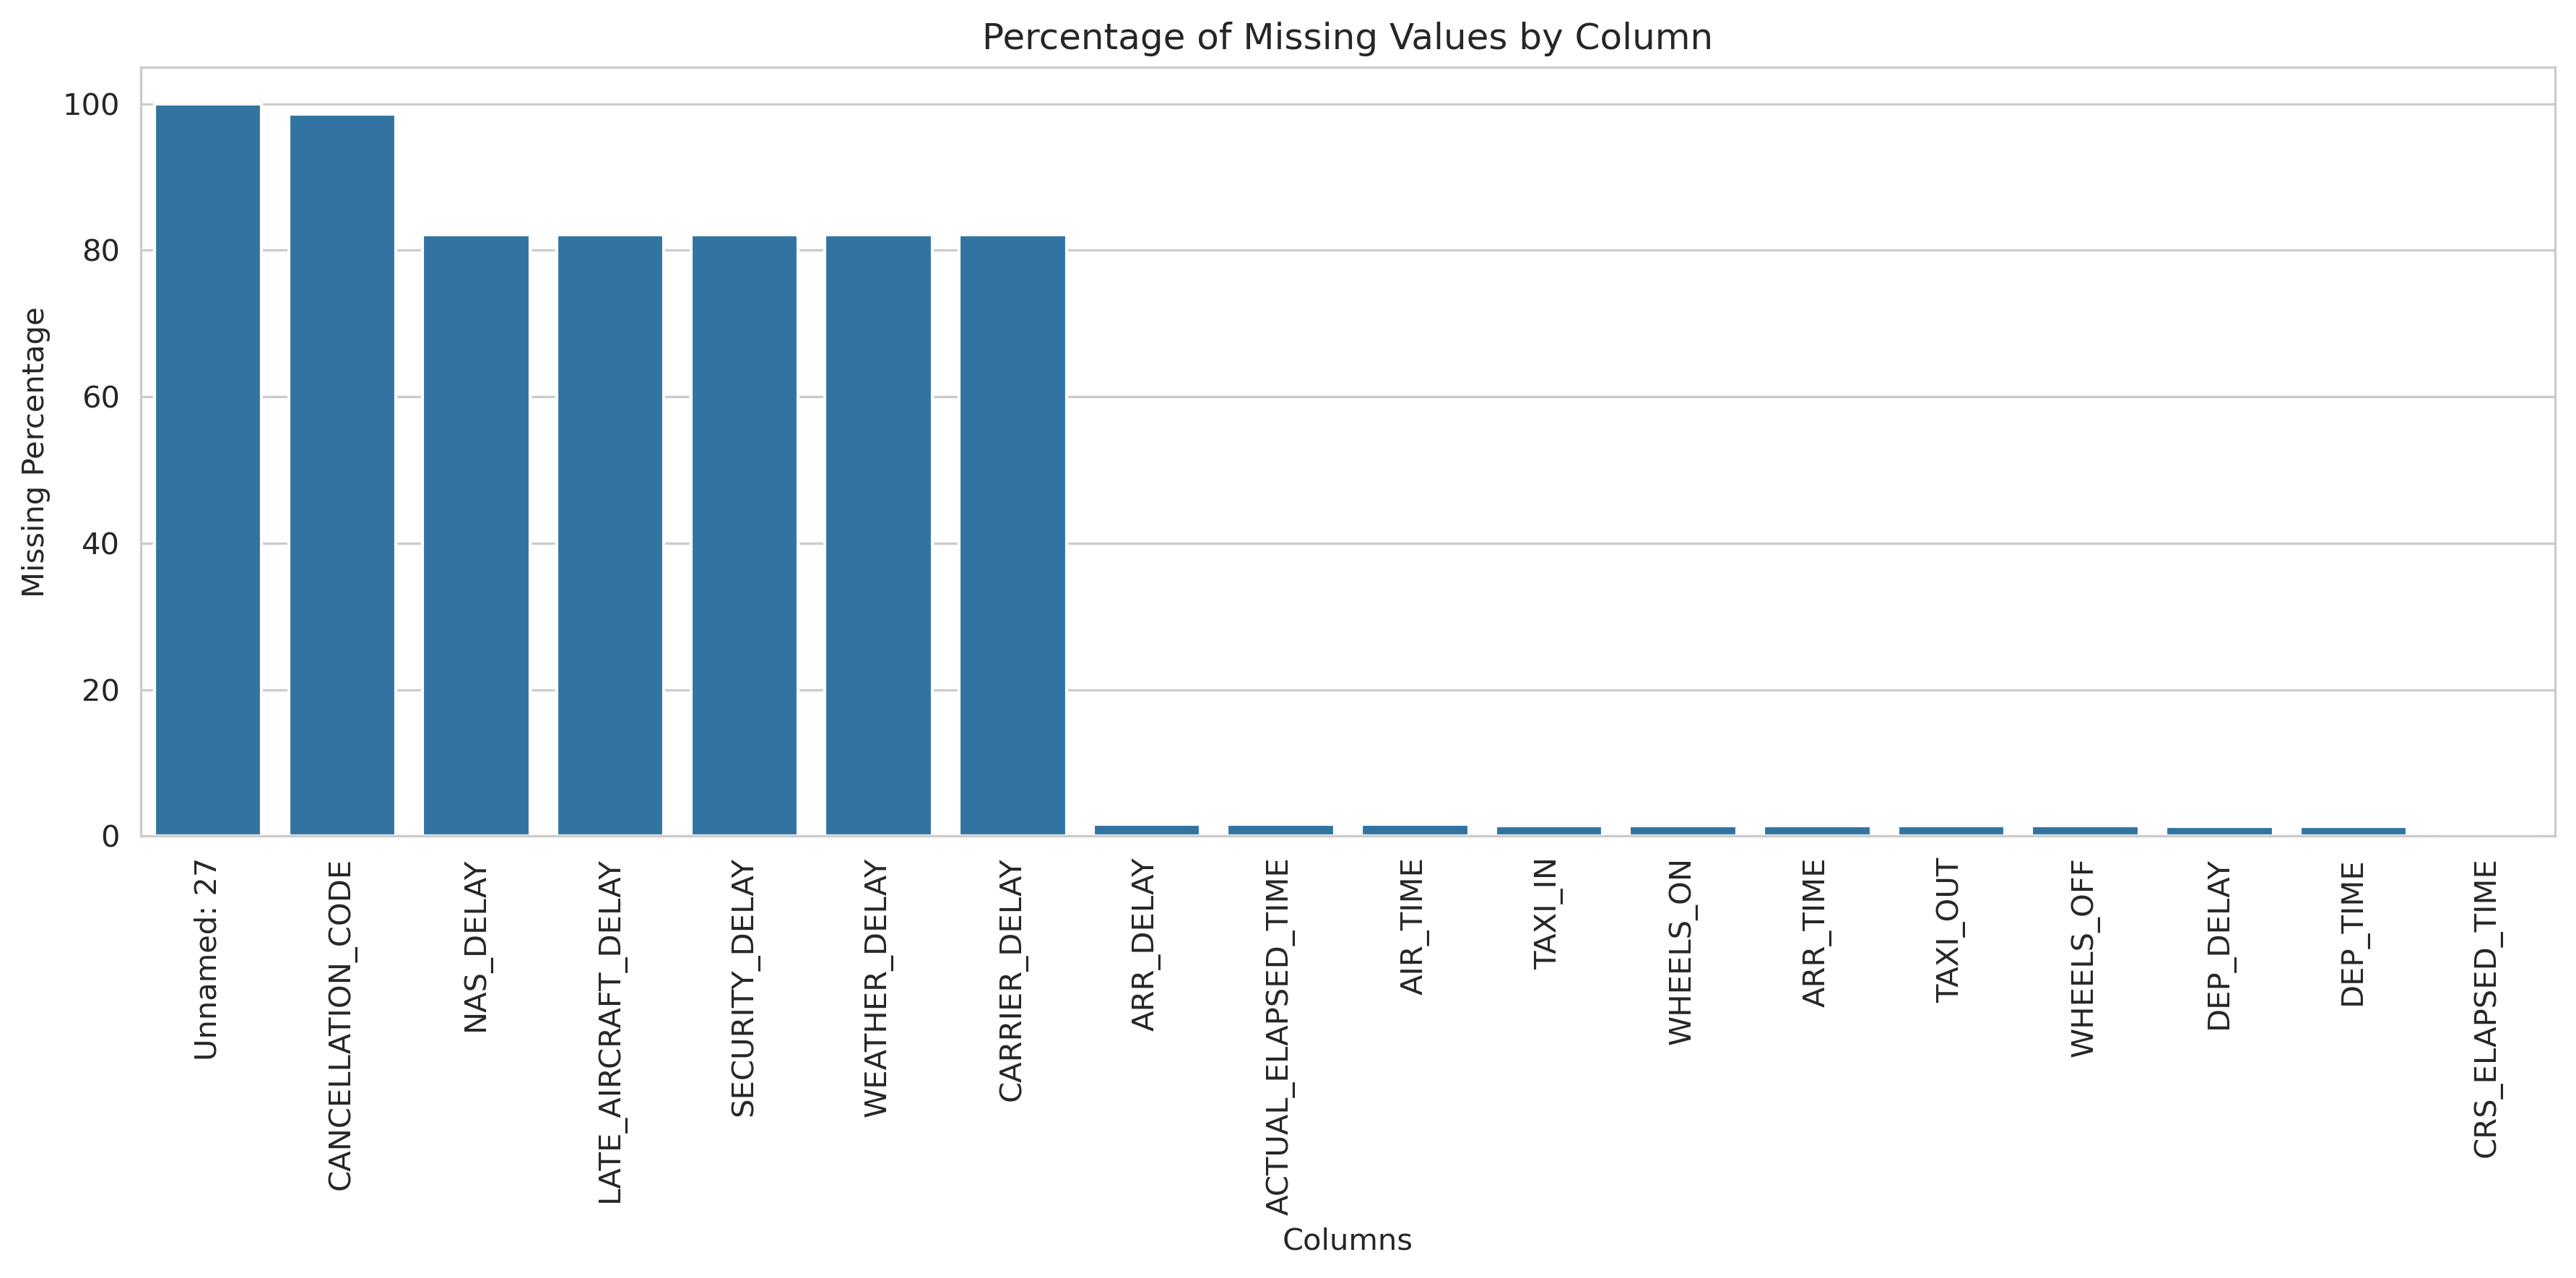
\includegraphics[width=0.85\textwidth]{figures/missing_values.png}
    \caption{Percentage of missing values across all columns. The \texttt{Unnamed: 27} column is entirely empty. Delay cause variables are missing for approximately 82\% of records, as they are only populated for flights with reported delays.}
\end{figure}

Key observations:
\begin{itemize}
    \item \texttt{Unnamed: 27}: 100\% missing (removed)
    \item \texttt{CANCELLATION\_CODE}: 98.6\% missing (only populated for cancelled flights, $\sim$1.4\%)
    \item Delay cause variables (\texttt{CARRIER\_DELAY}, \texttt{WEATHER\_DELAY}, \texttt{NAS\_DELAY}, \texttt{SECURITY\_DELAY}, \texttt{LATE\_AIRCRAFT\_DELAY}): $\sim$82\% missing
    \item \texttt{ARR\_DELAY}: 1.6\% missing
    \item \texttt{DEP\_DELAY}: minimal missing values
\end{itemize}

The missingness follows an expected operational pattern: delay causes are logged only when delays exceed reporting thresholds, and arrival-related fields are absent for cancelled or diverted flights.

\subsection{Summary Statistics}

The descriptive statistics highlight several notable characteristics:
\begin{itemize}
    \item Mean departure delay: 9.35 minutes; mean arrival delay: 4.09 minutes
    \item Median delays are negative (-2 minutes departure, -6 minutes arrival), indicating that most flights depart and arrive slightly ahead of schedule
    \item Maximum delays exceed 2,000 minutes, indicating severe outlier events
    \item Cancellation rate: 1.39\%; Diversion rate: 0.24\%
    \item Average flight distance: 843 km
\end{itemize}

\section{Univariate Analysis}

\subsection{Flight Volume}

Flight volume remained relatively stable across the three years:

\begin{figure}[H]
    \centering
    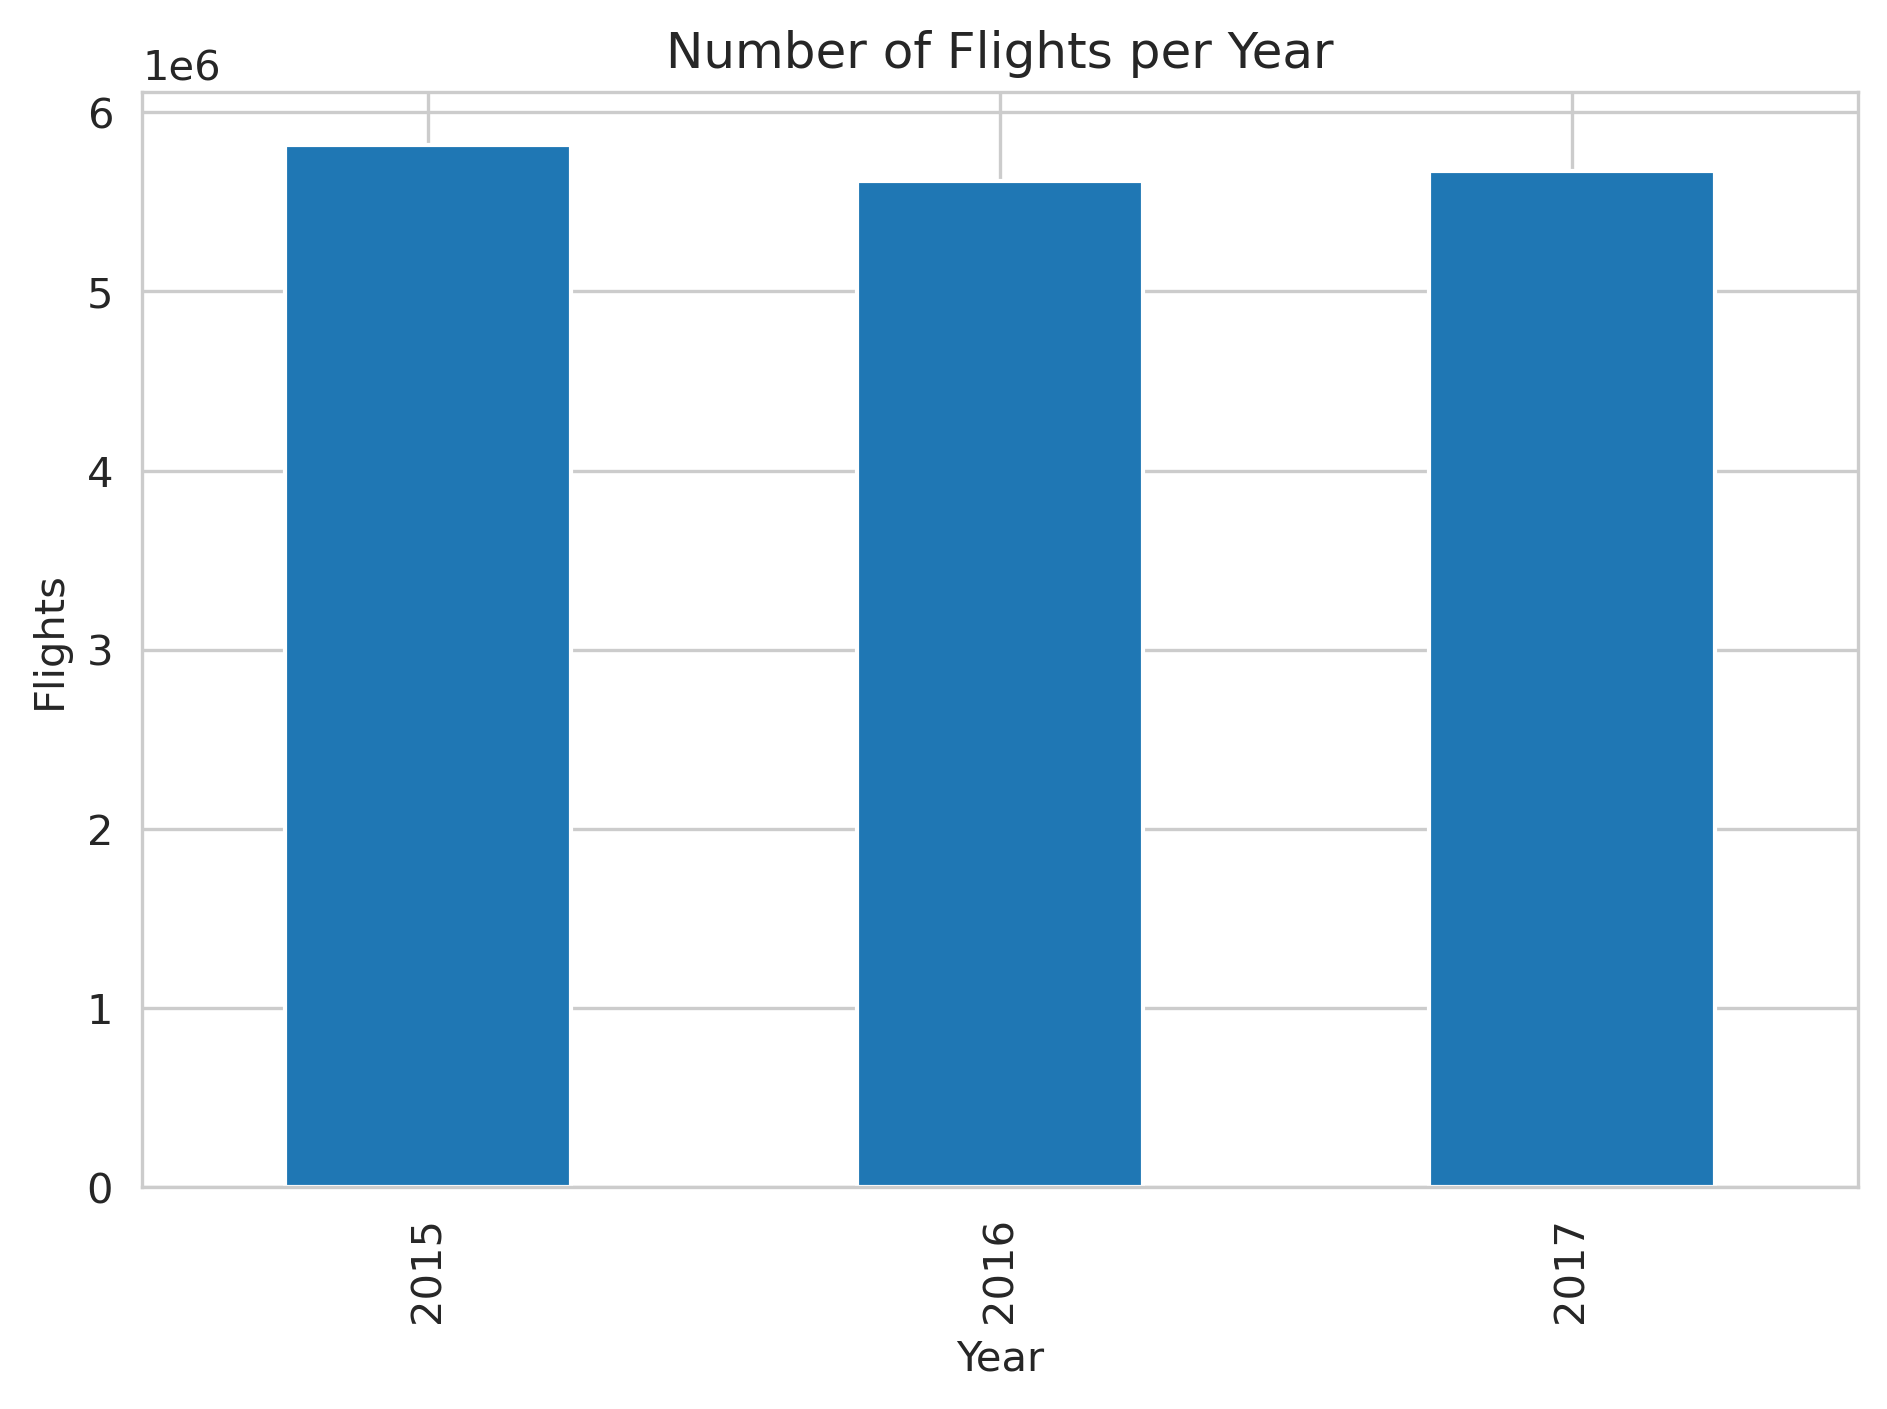
\includegraphics[width=0.85\textwidth]{figures/yearly_flights.png}
    \caption{Total number of flights per year (2015--2017).}
\end{figure}

\begin{figure}[H]
    \centering
    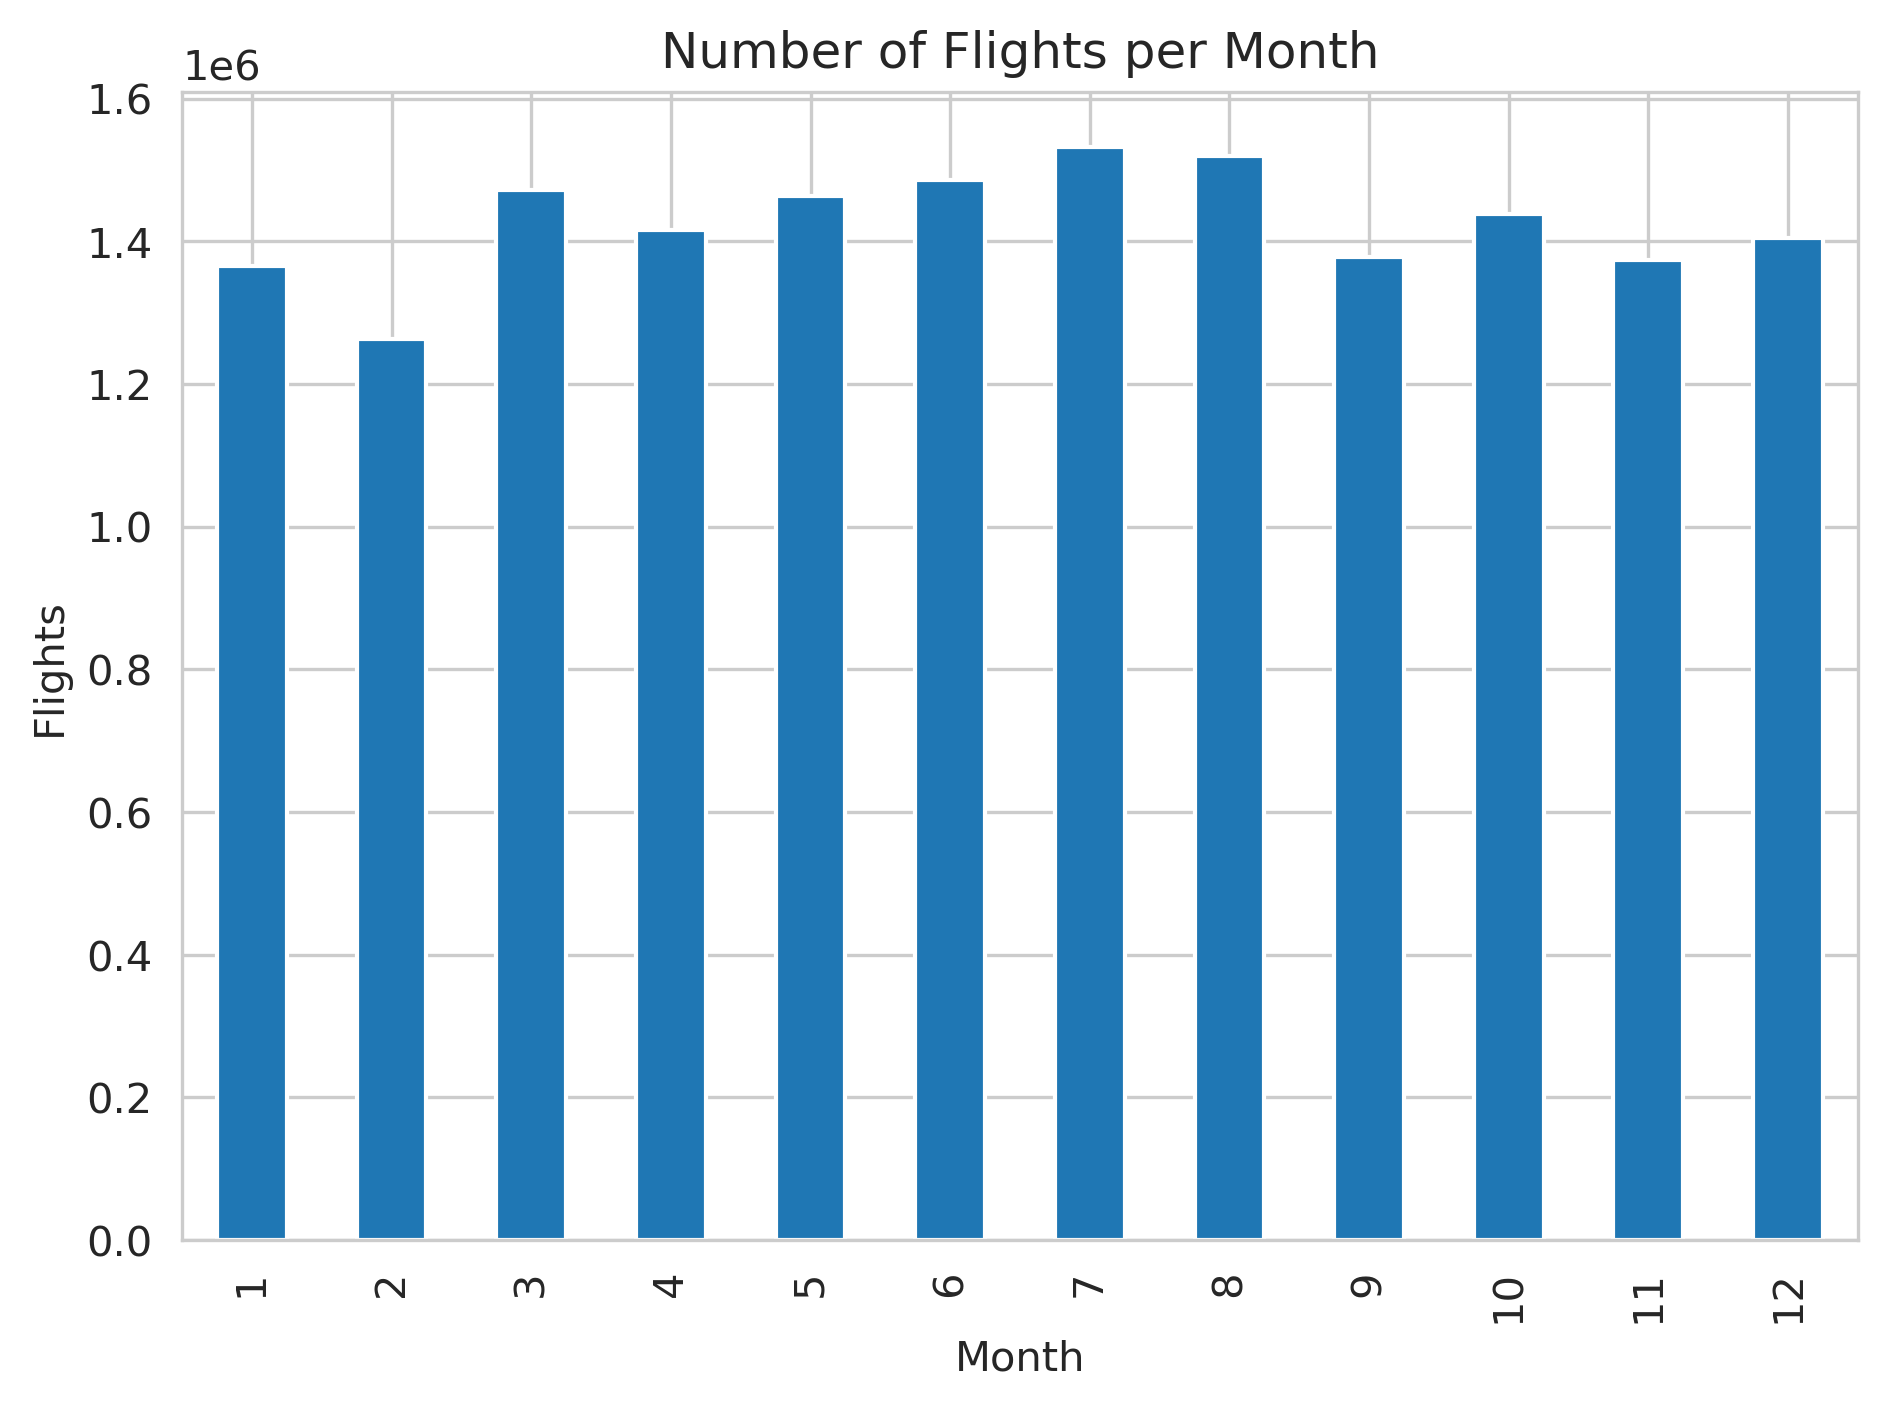
\includegraphics[width=0.85\textwidth]{figures/monthly_flights.png}
    \caption{Monthly flight distribution showing peak traffic during summer months (June--August).}
\end{figure}

\subsection{Delay Distributions}

Both arrival and departure delays exhibit strong right-skewness with long tails:

\begin{figure}[H]
    \centering
    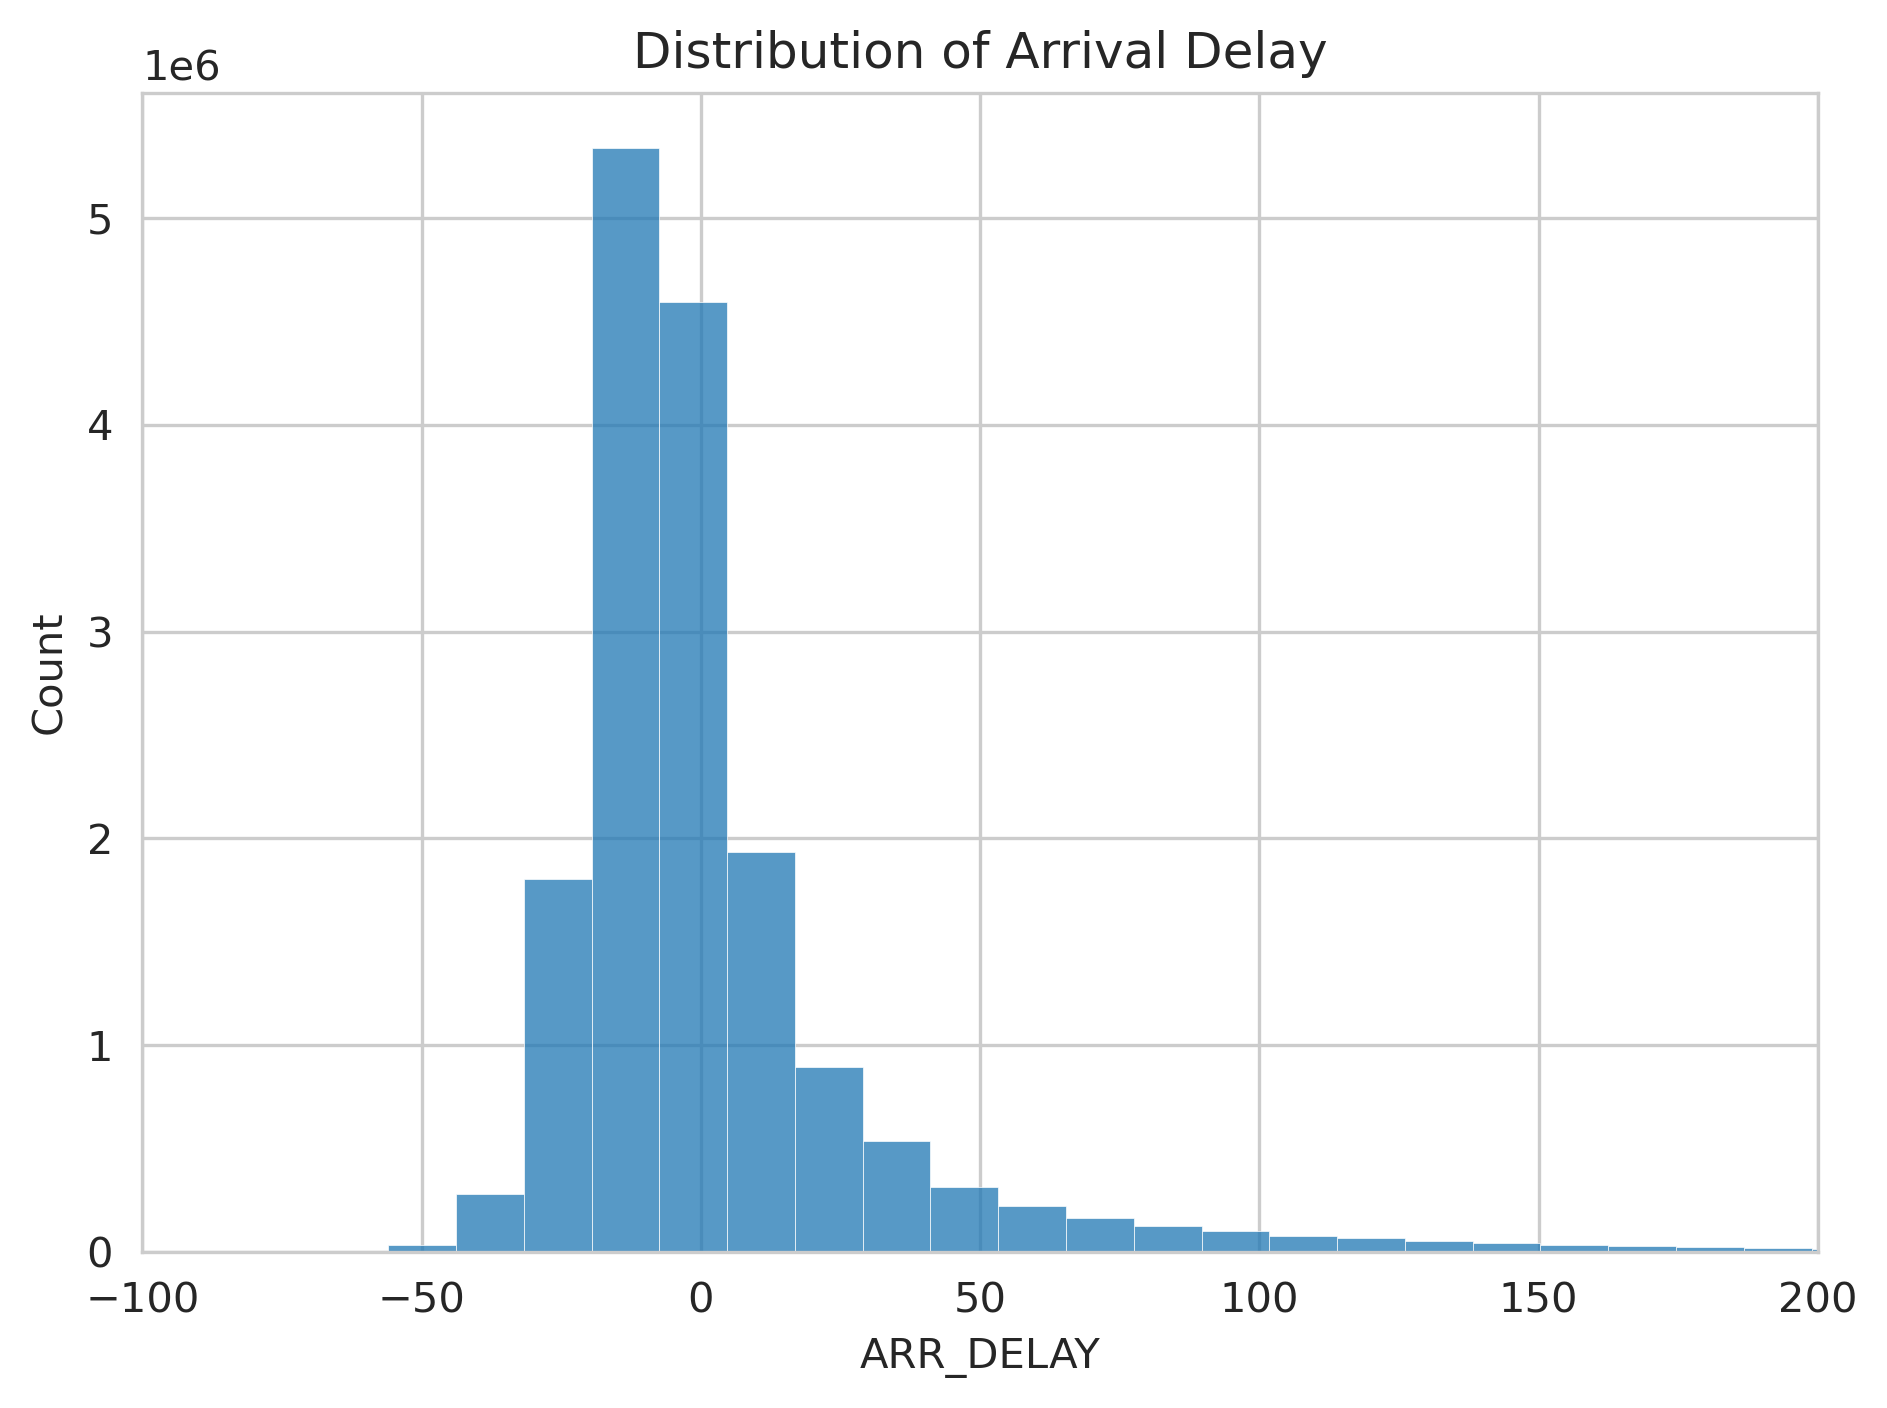
\includegraphics[width=0.85\textwidth]{figures/arr_delay_hist.png}
    \caption{Distribution of arrival delay (minutes). The distribution is centered near zero with a prominent left peak indicating early arrivals.}
\end{figure}

\begin{figure}[H]
    \centering
    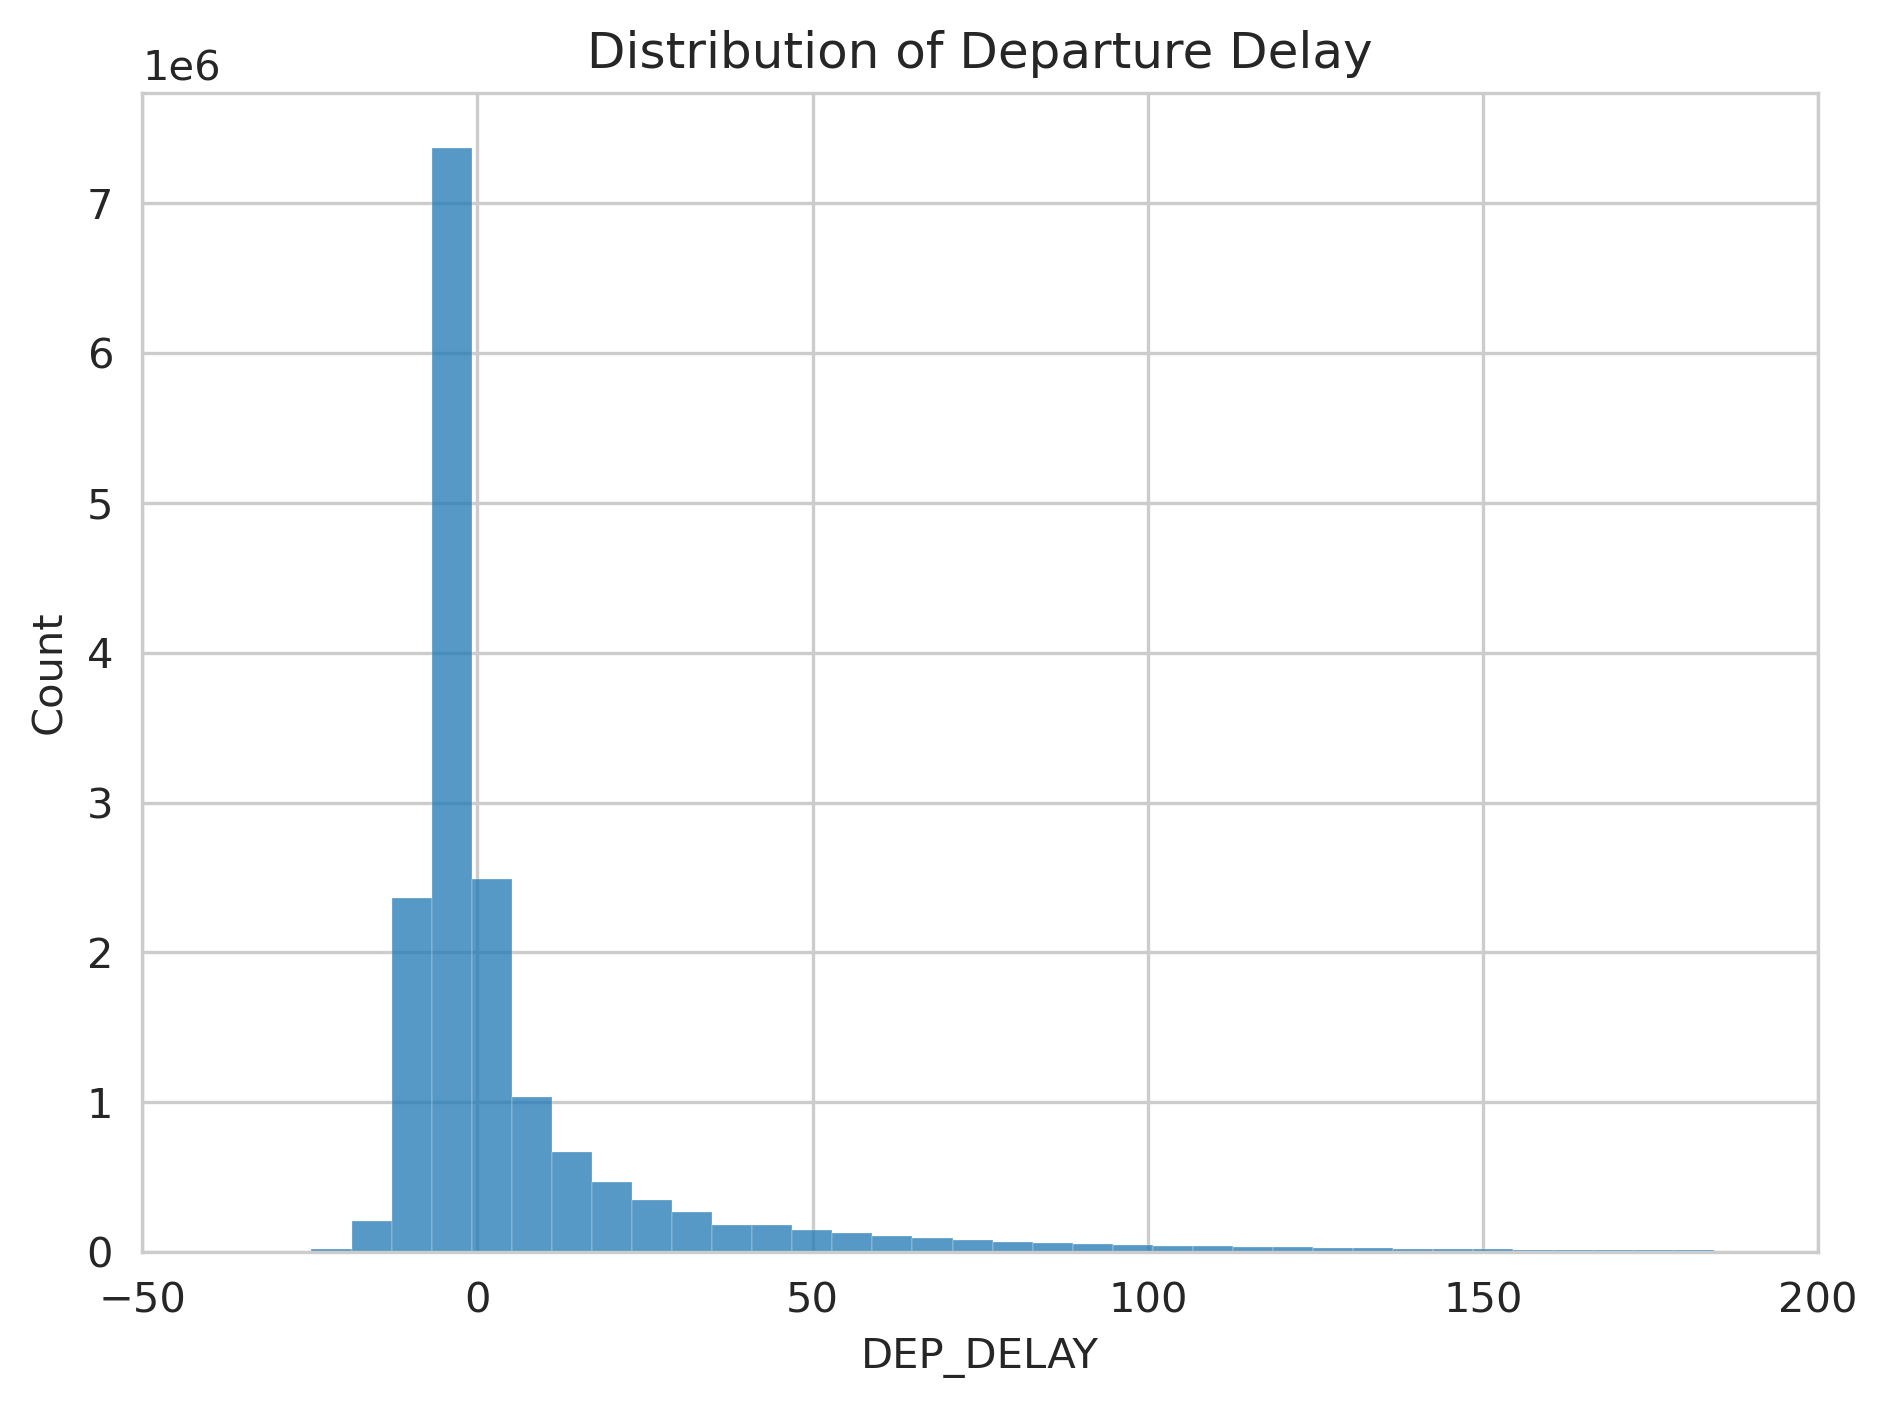
\includegraphics[width=0.85\textwidth]{figures/dep_delay_hist.png}
    \caption{Distribution of departure delay (minutes). Similar right-skewed pattern with a concentration near zero.}
\end{figure}

\subsection{Distance Distribution}

\begin{figure}[H]
    \centering
    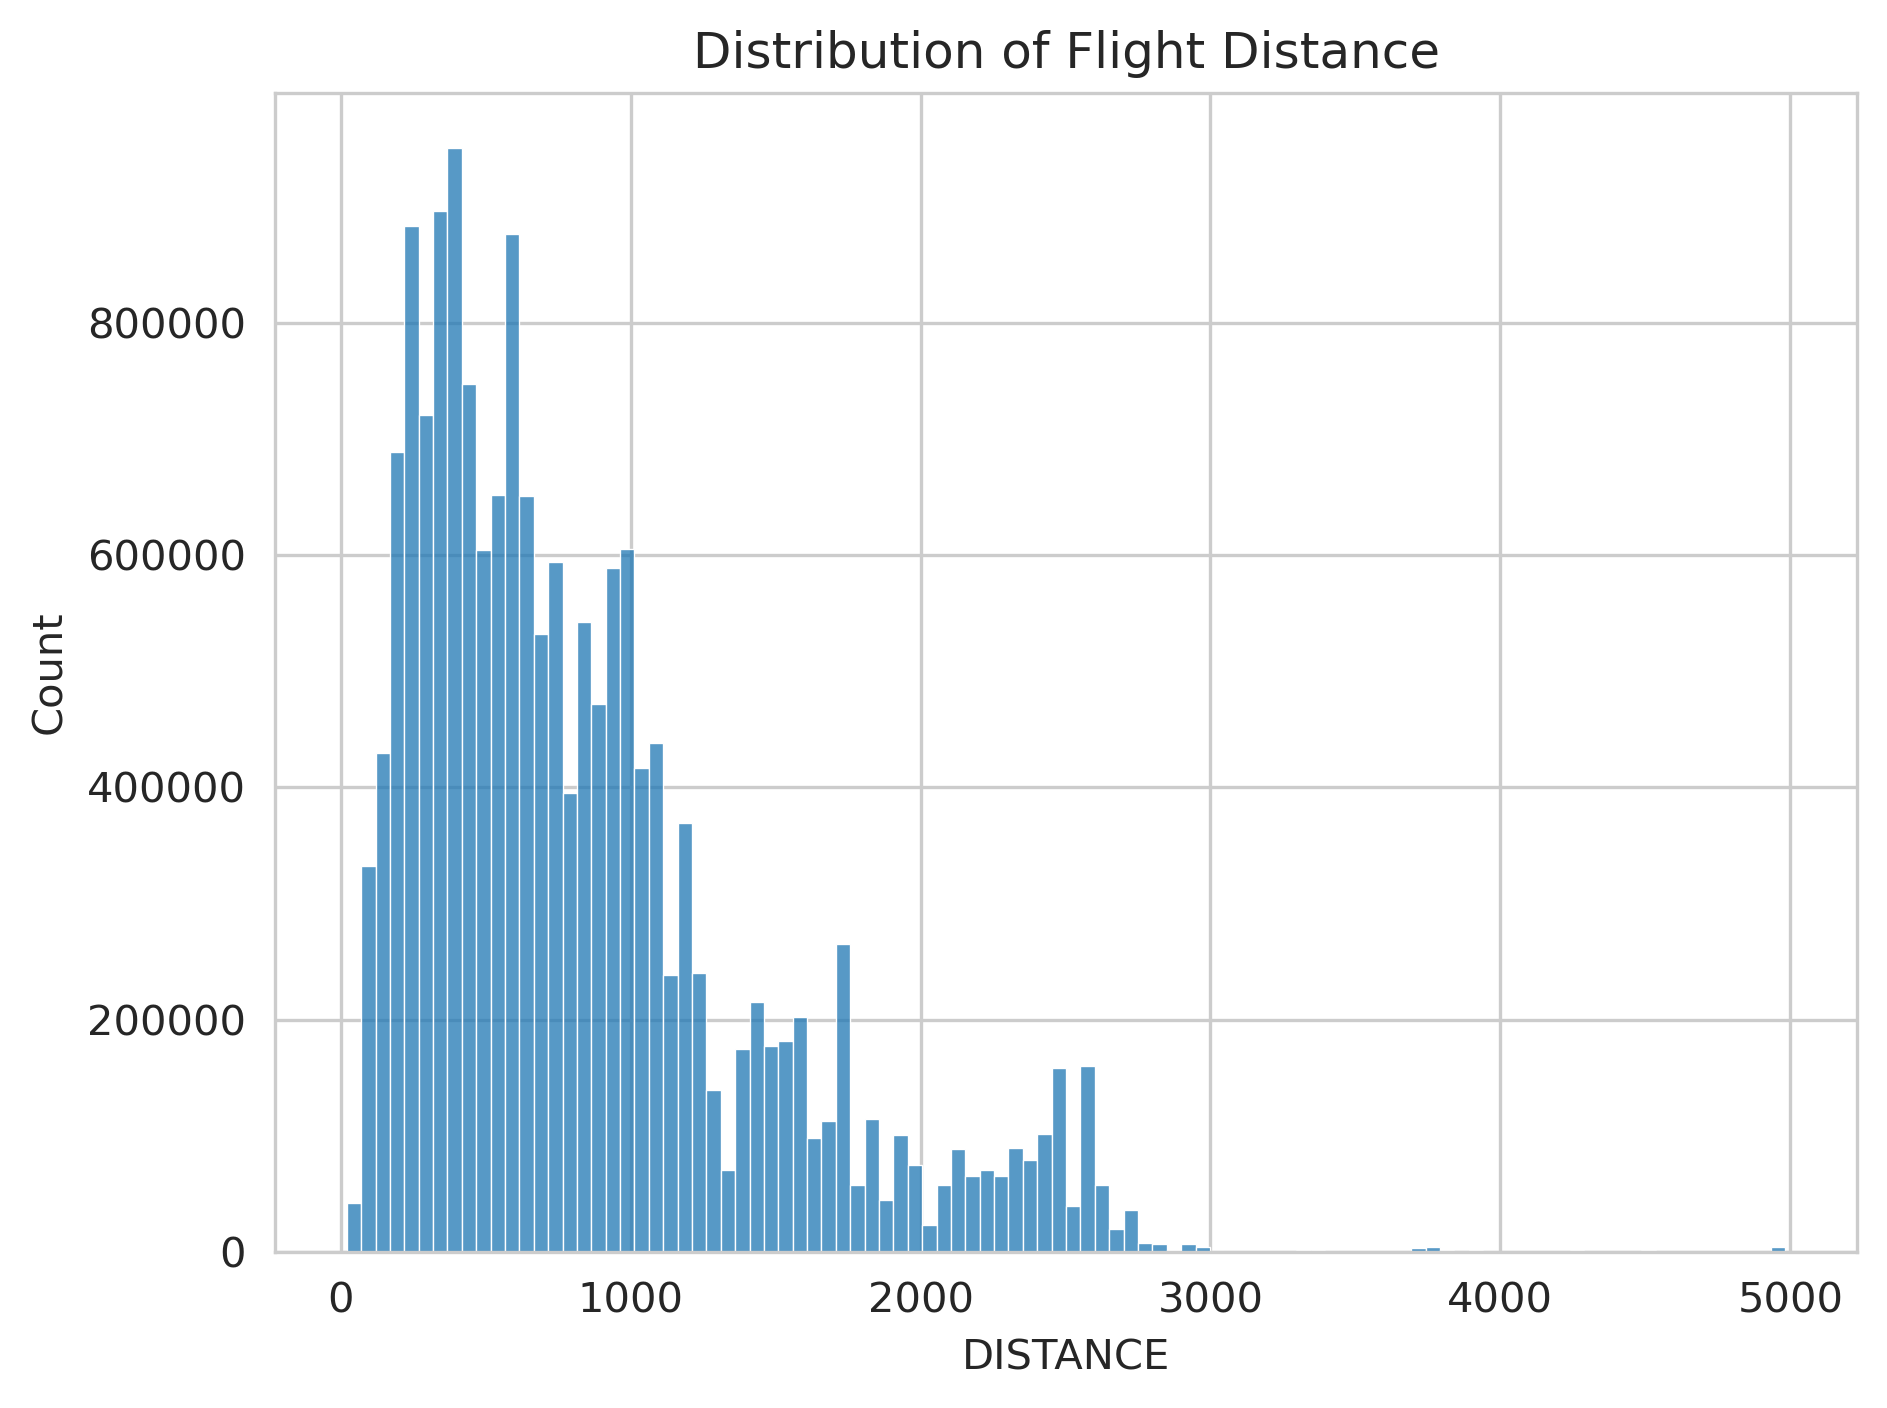
\includegraphics[width=0.85\textwidth]{figures/distance_hist.png}
    \caption{Flight distance distribution. Most flights are short- to medium-haul, concentrated under 2,000 km.}
\end{figure}

The majority of flights operate on short- to medium-haul routes (under 1,500 km), consistent with the domestic nature of the dataset.

\section{Categorical Analysis}

\subsection{Carrier Distribution}

\begin{figure}[H]
    \centering
    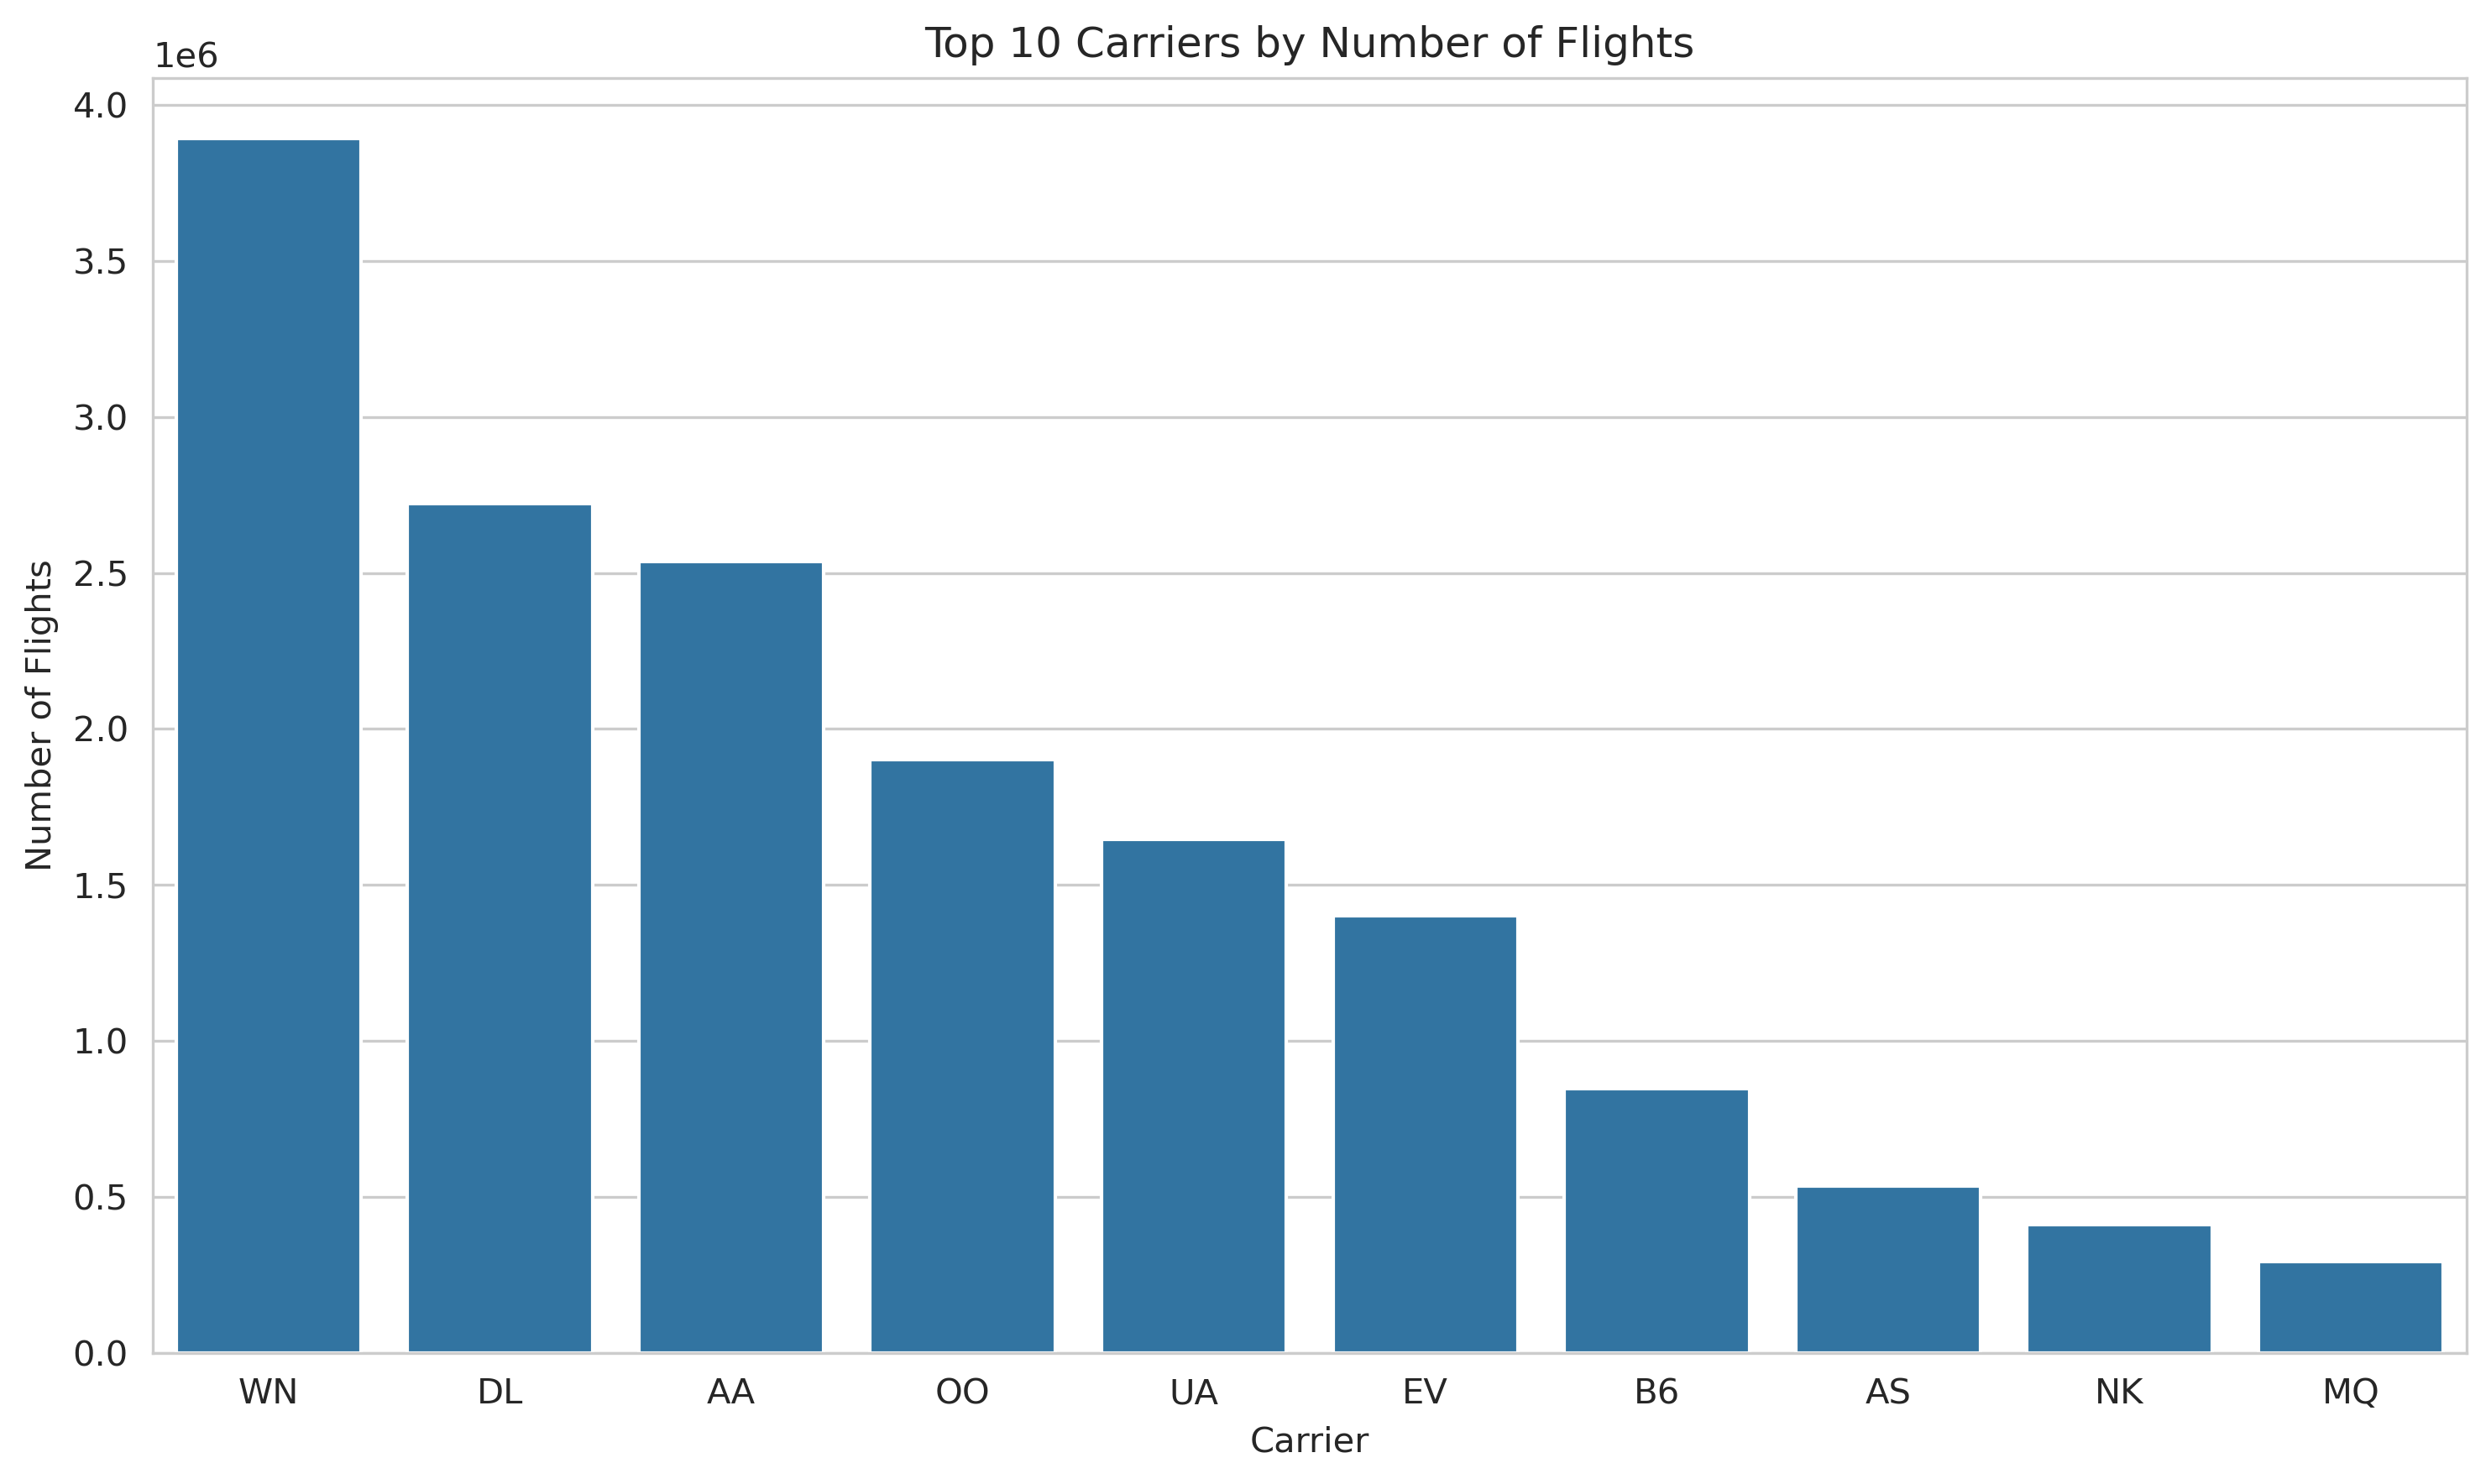
\includegraphics[width=0.85\textwidth]{figures/carrier_counts.png}
    \caption{Top 10 carriers by total number of flights. Southwest Airlines (WN) is the dominant carrier.}
\end{figure}

The market is dominated by a few major carriers:
\begin{itemize}
    \item WN (Southwest Airlines) operates the largest share of flights
    \item DL (Delta Air Lines) and AA (American Airlines) follow closely
    \item The top 5 carriers account for the majority of all domestic traffic
\end{itemize}

\subsection{Airport Activity}

\begin{figure}[H]
    \centering
    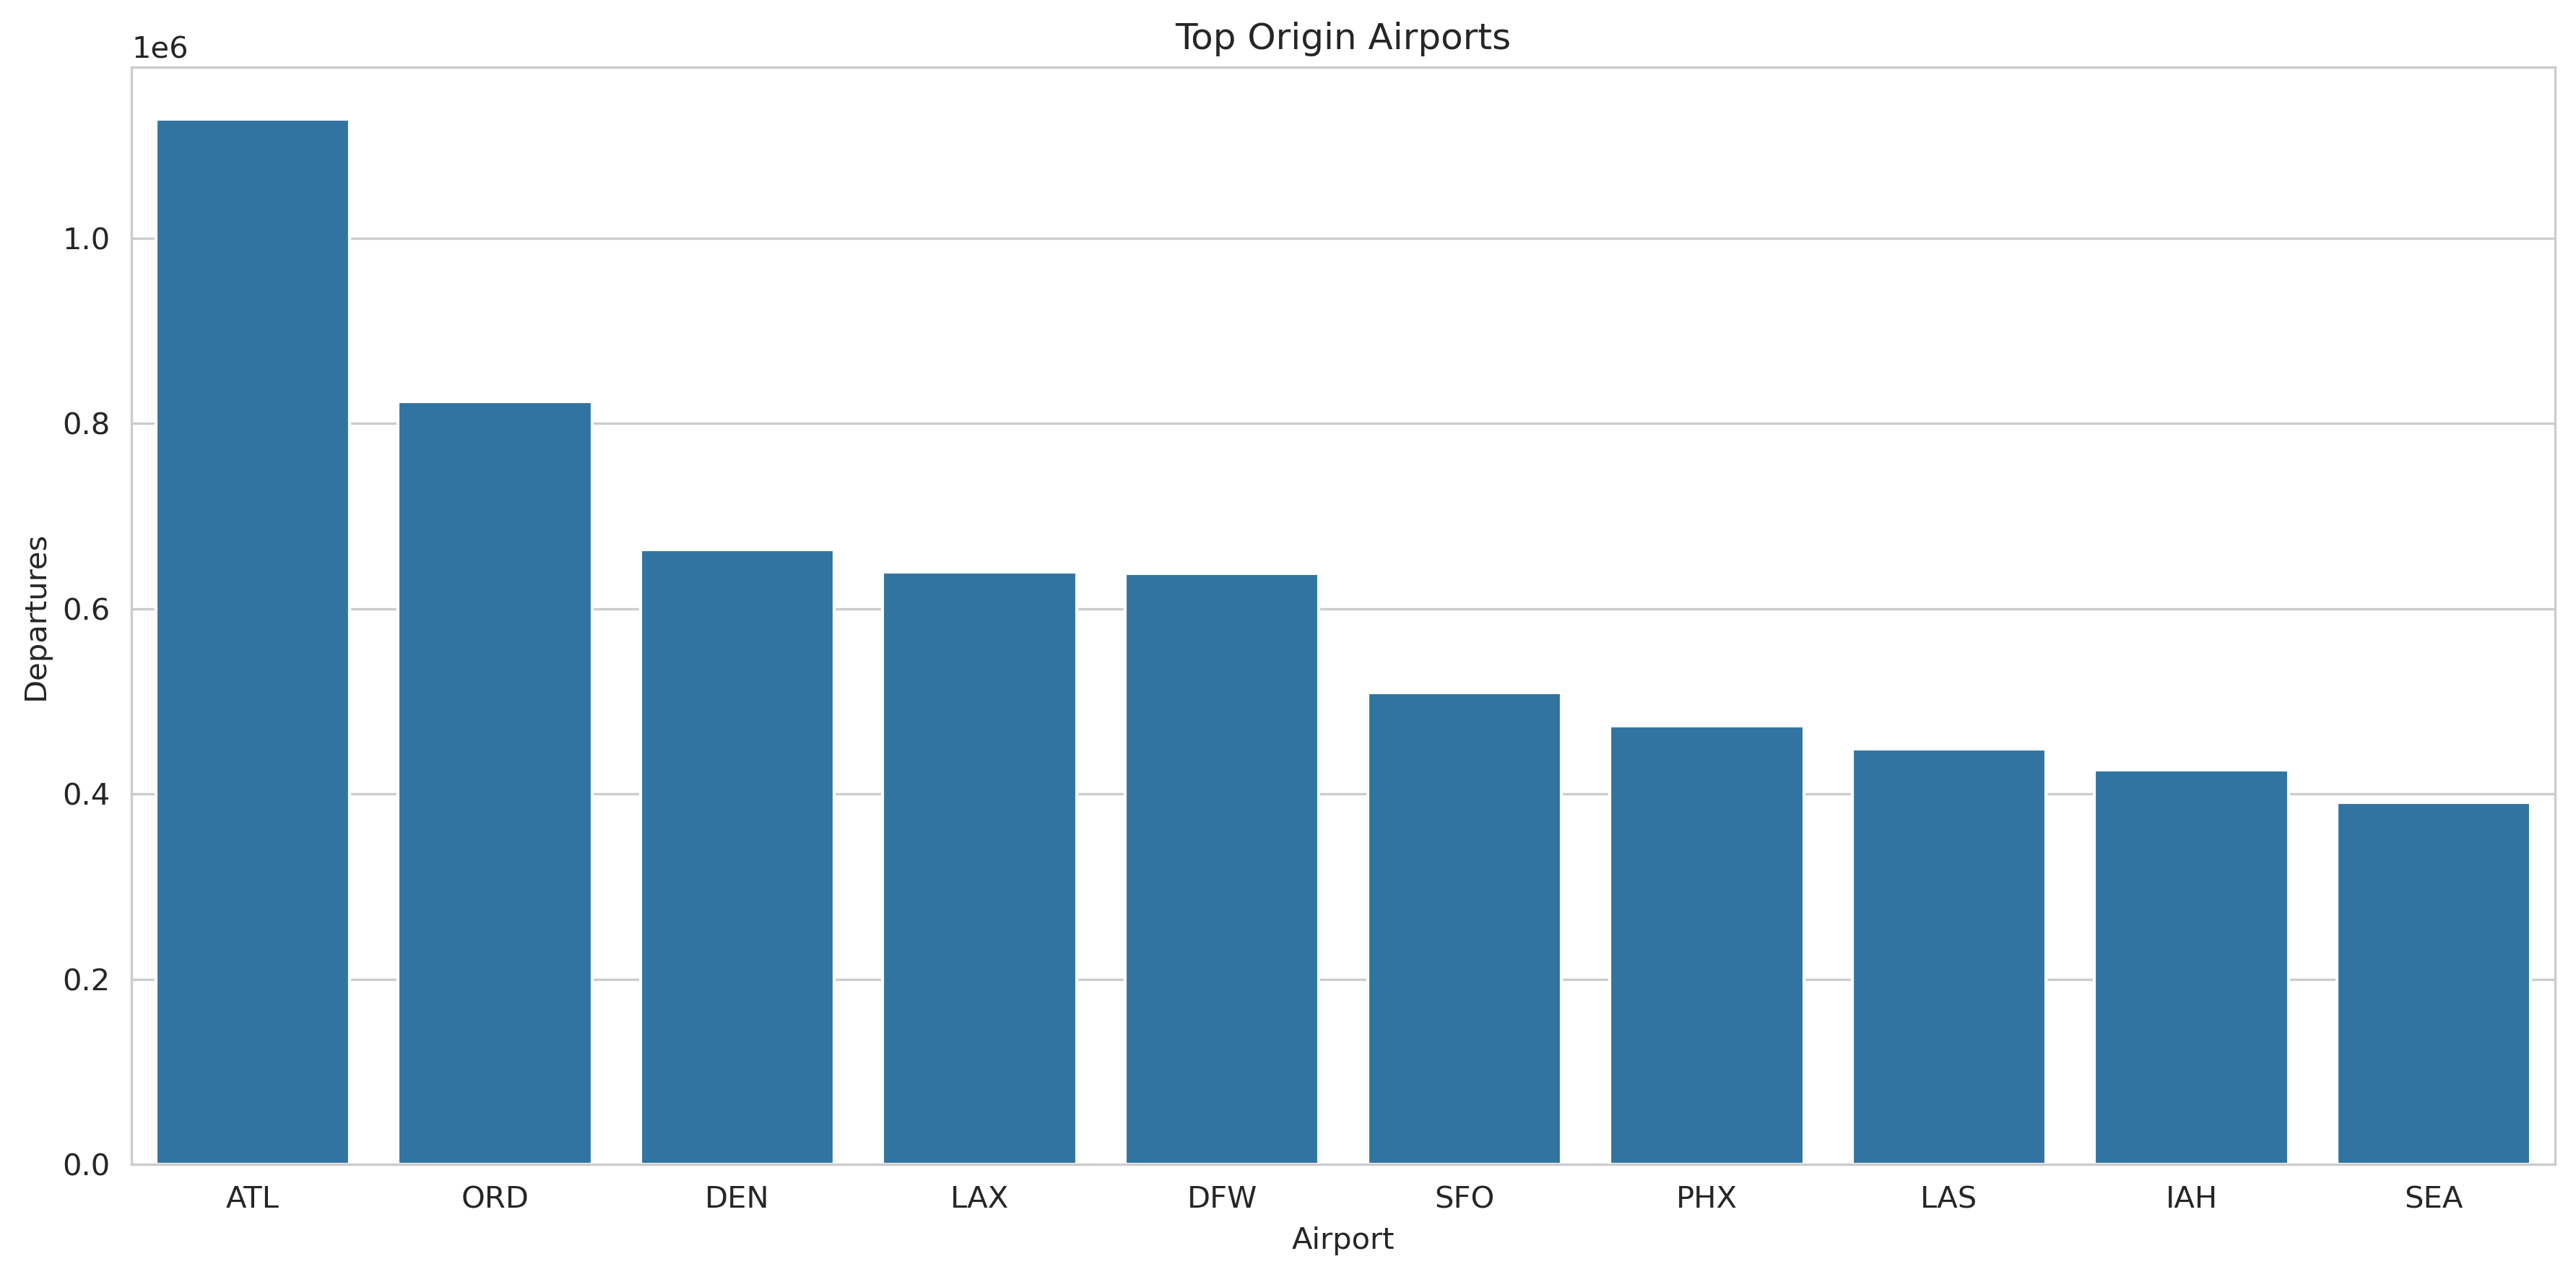
\includegraphics[width=0.85\textwidth]{figures/airport_counts.png}
    \caption{Top 10 busiest origin airports. ATL (Atlanta), ORD (Chicago O'Hare), and DEN (Denver) lead in traffic volume.}
\end{figure}

Major hub airports dominate departure volumes, with ATL, ORD, DEN, DFW, and LAX among the busiest.

\subsection{Cancellations and Diversions}

The overall cancellation rate is 1.39\% and the diversion rate is 0.24\%. While small in percentage terms, these represent hundreds of thousands of disrupted flights annually.

\section{Temporal Patterns}

\subsection{Yearly Trends}

\begin{figure}[H]
    \centering
    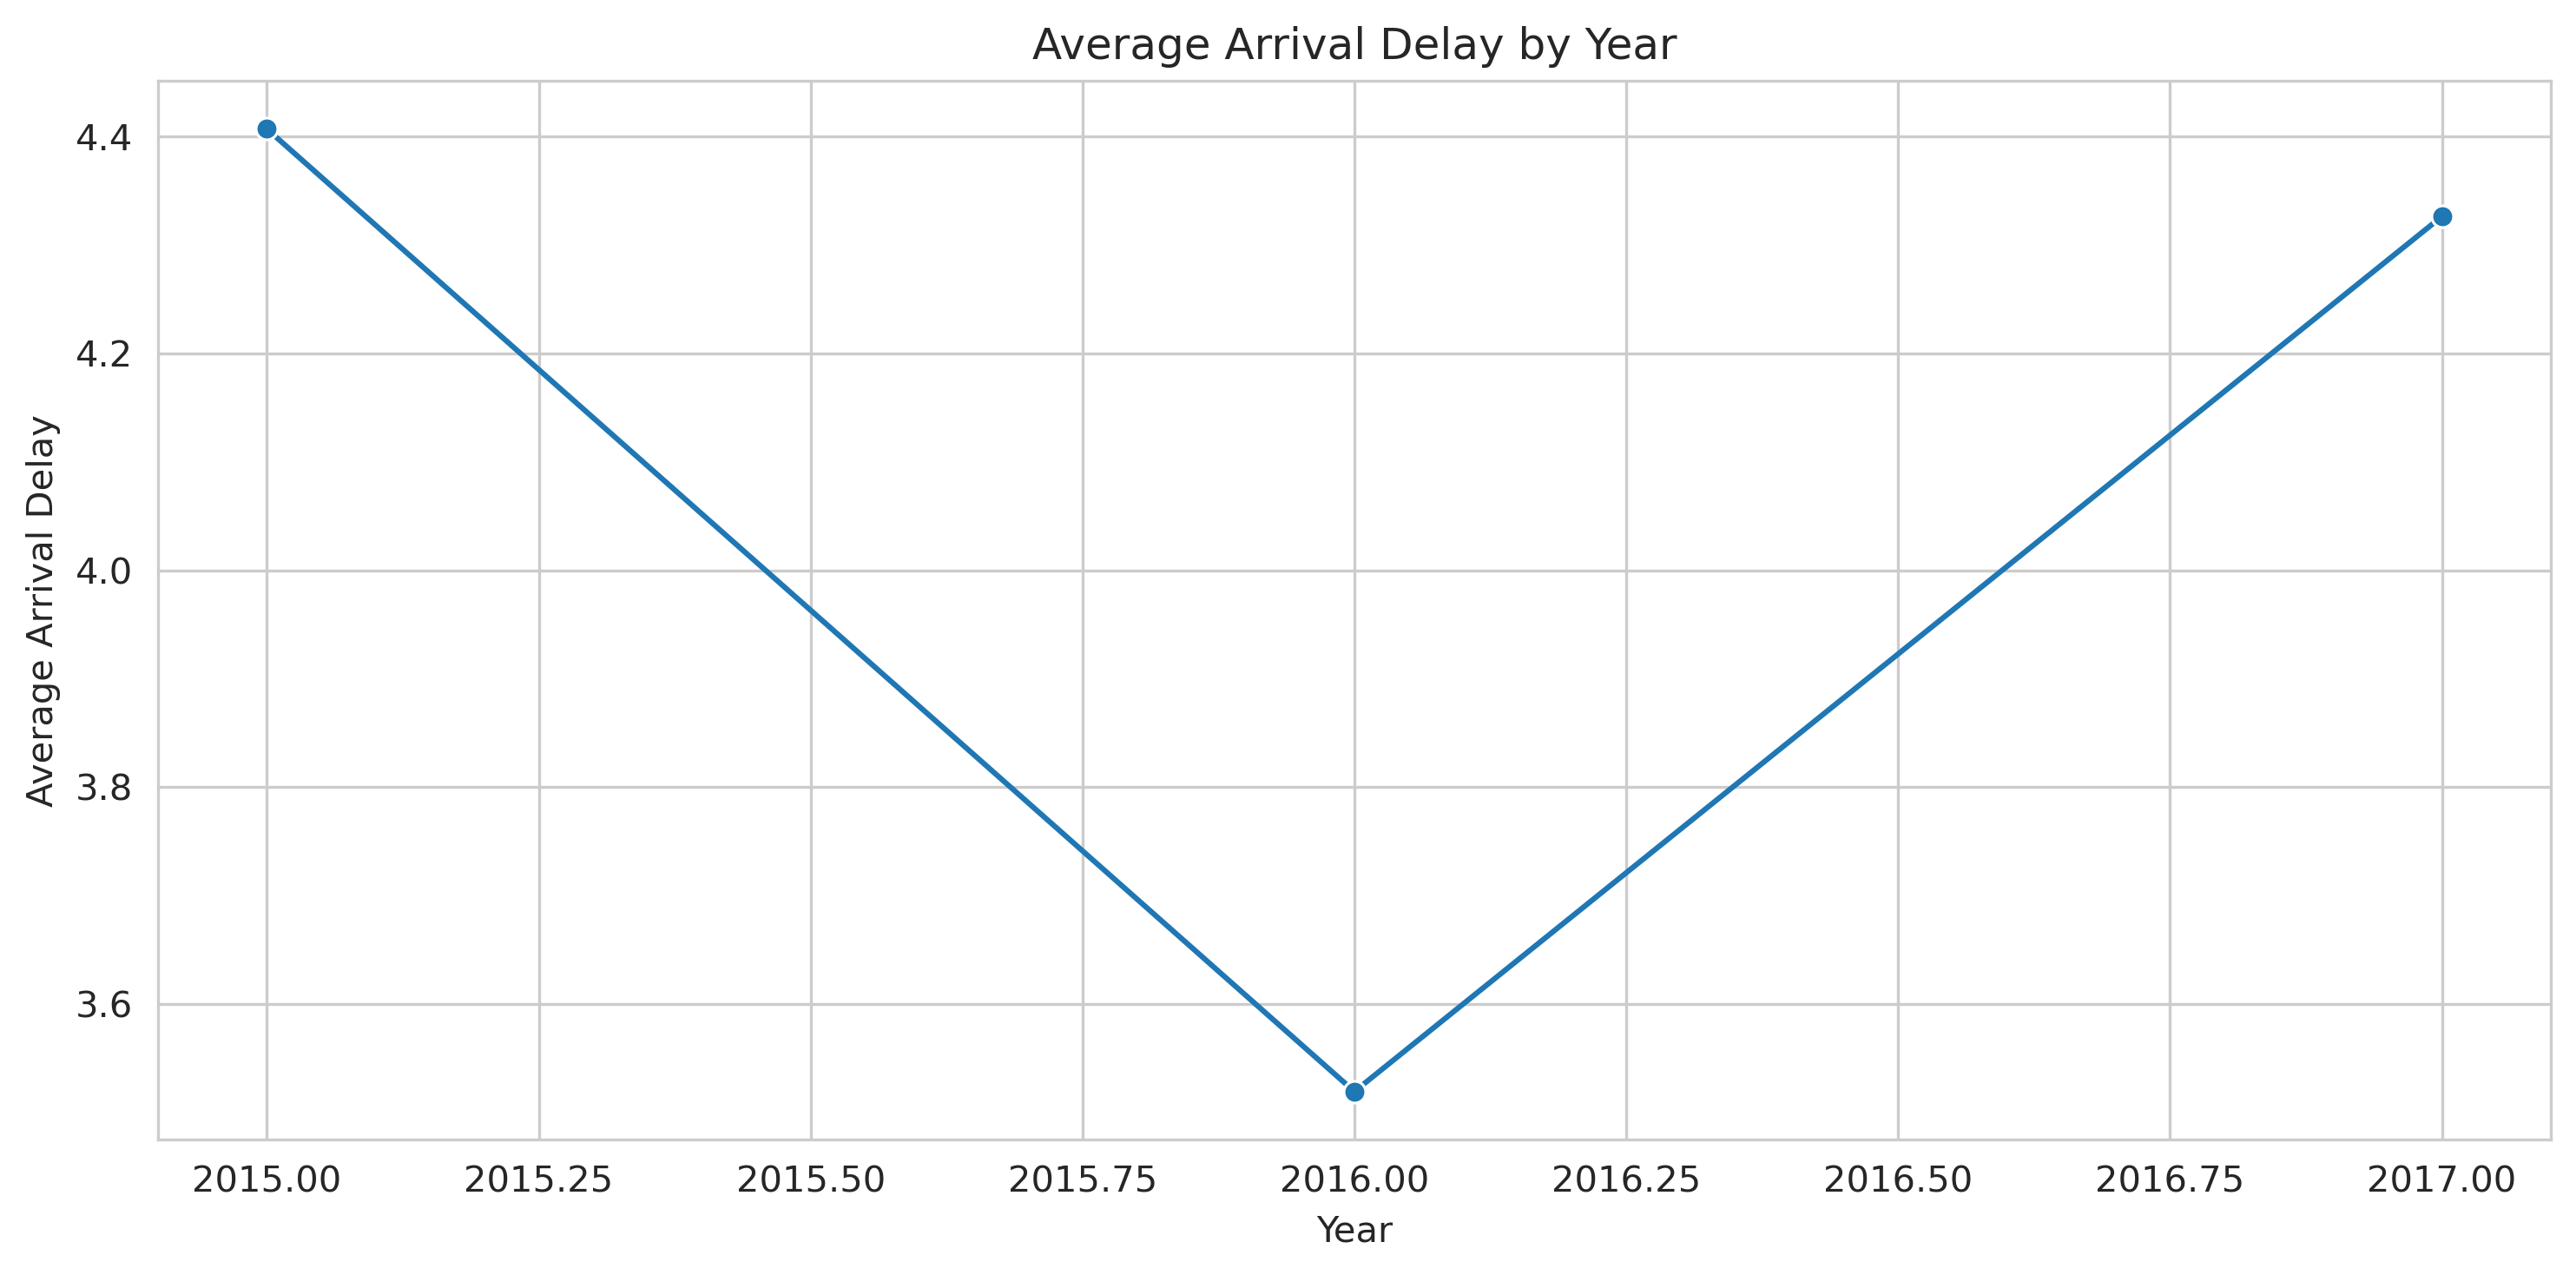
\includegraphics[width=0.85\textwidth]{figures/yearly_delay.png}
    \caption{Average arrival delay by year.}
\end{figure}

\begin{figure}[H]
    \centering
    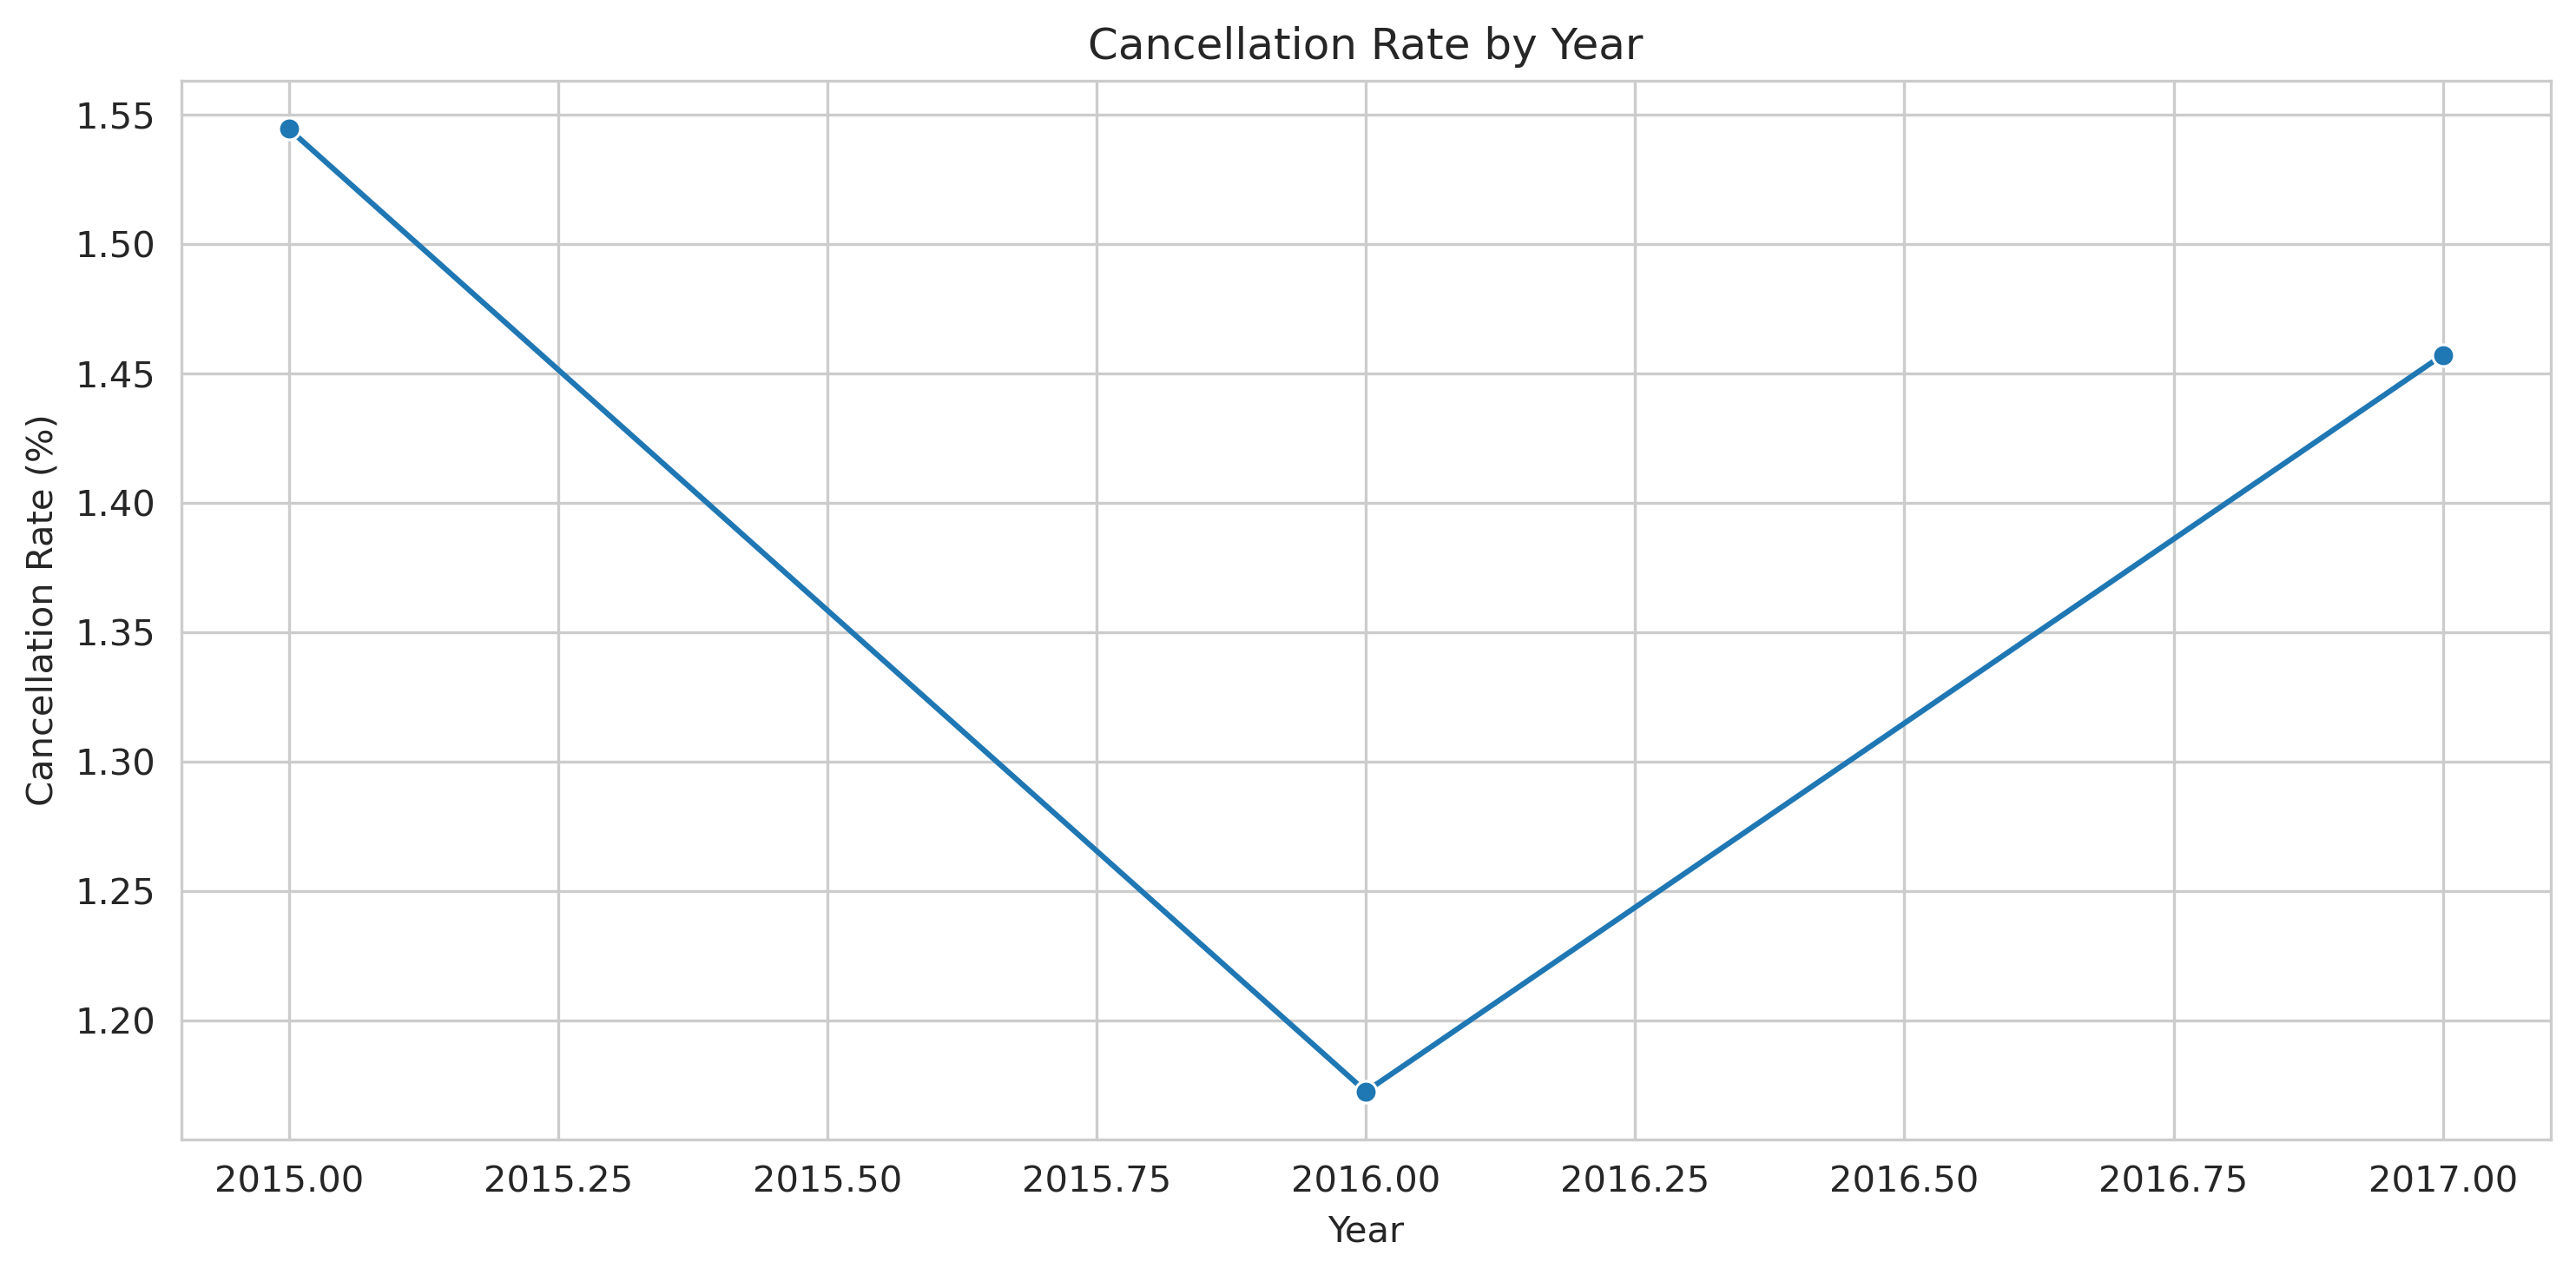
\includegraphics[width=0.85\textwidth]{figures/cancellation_rate.png}
    \caption{Cancellation rate by year.}
\end{figure}

\subsection{Weekly and Hourly Patterns}

\begin{figure}[H]
    \centering
    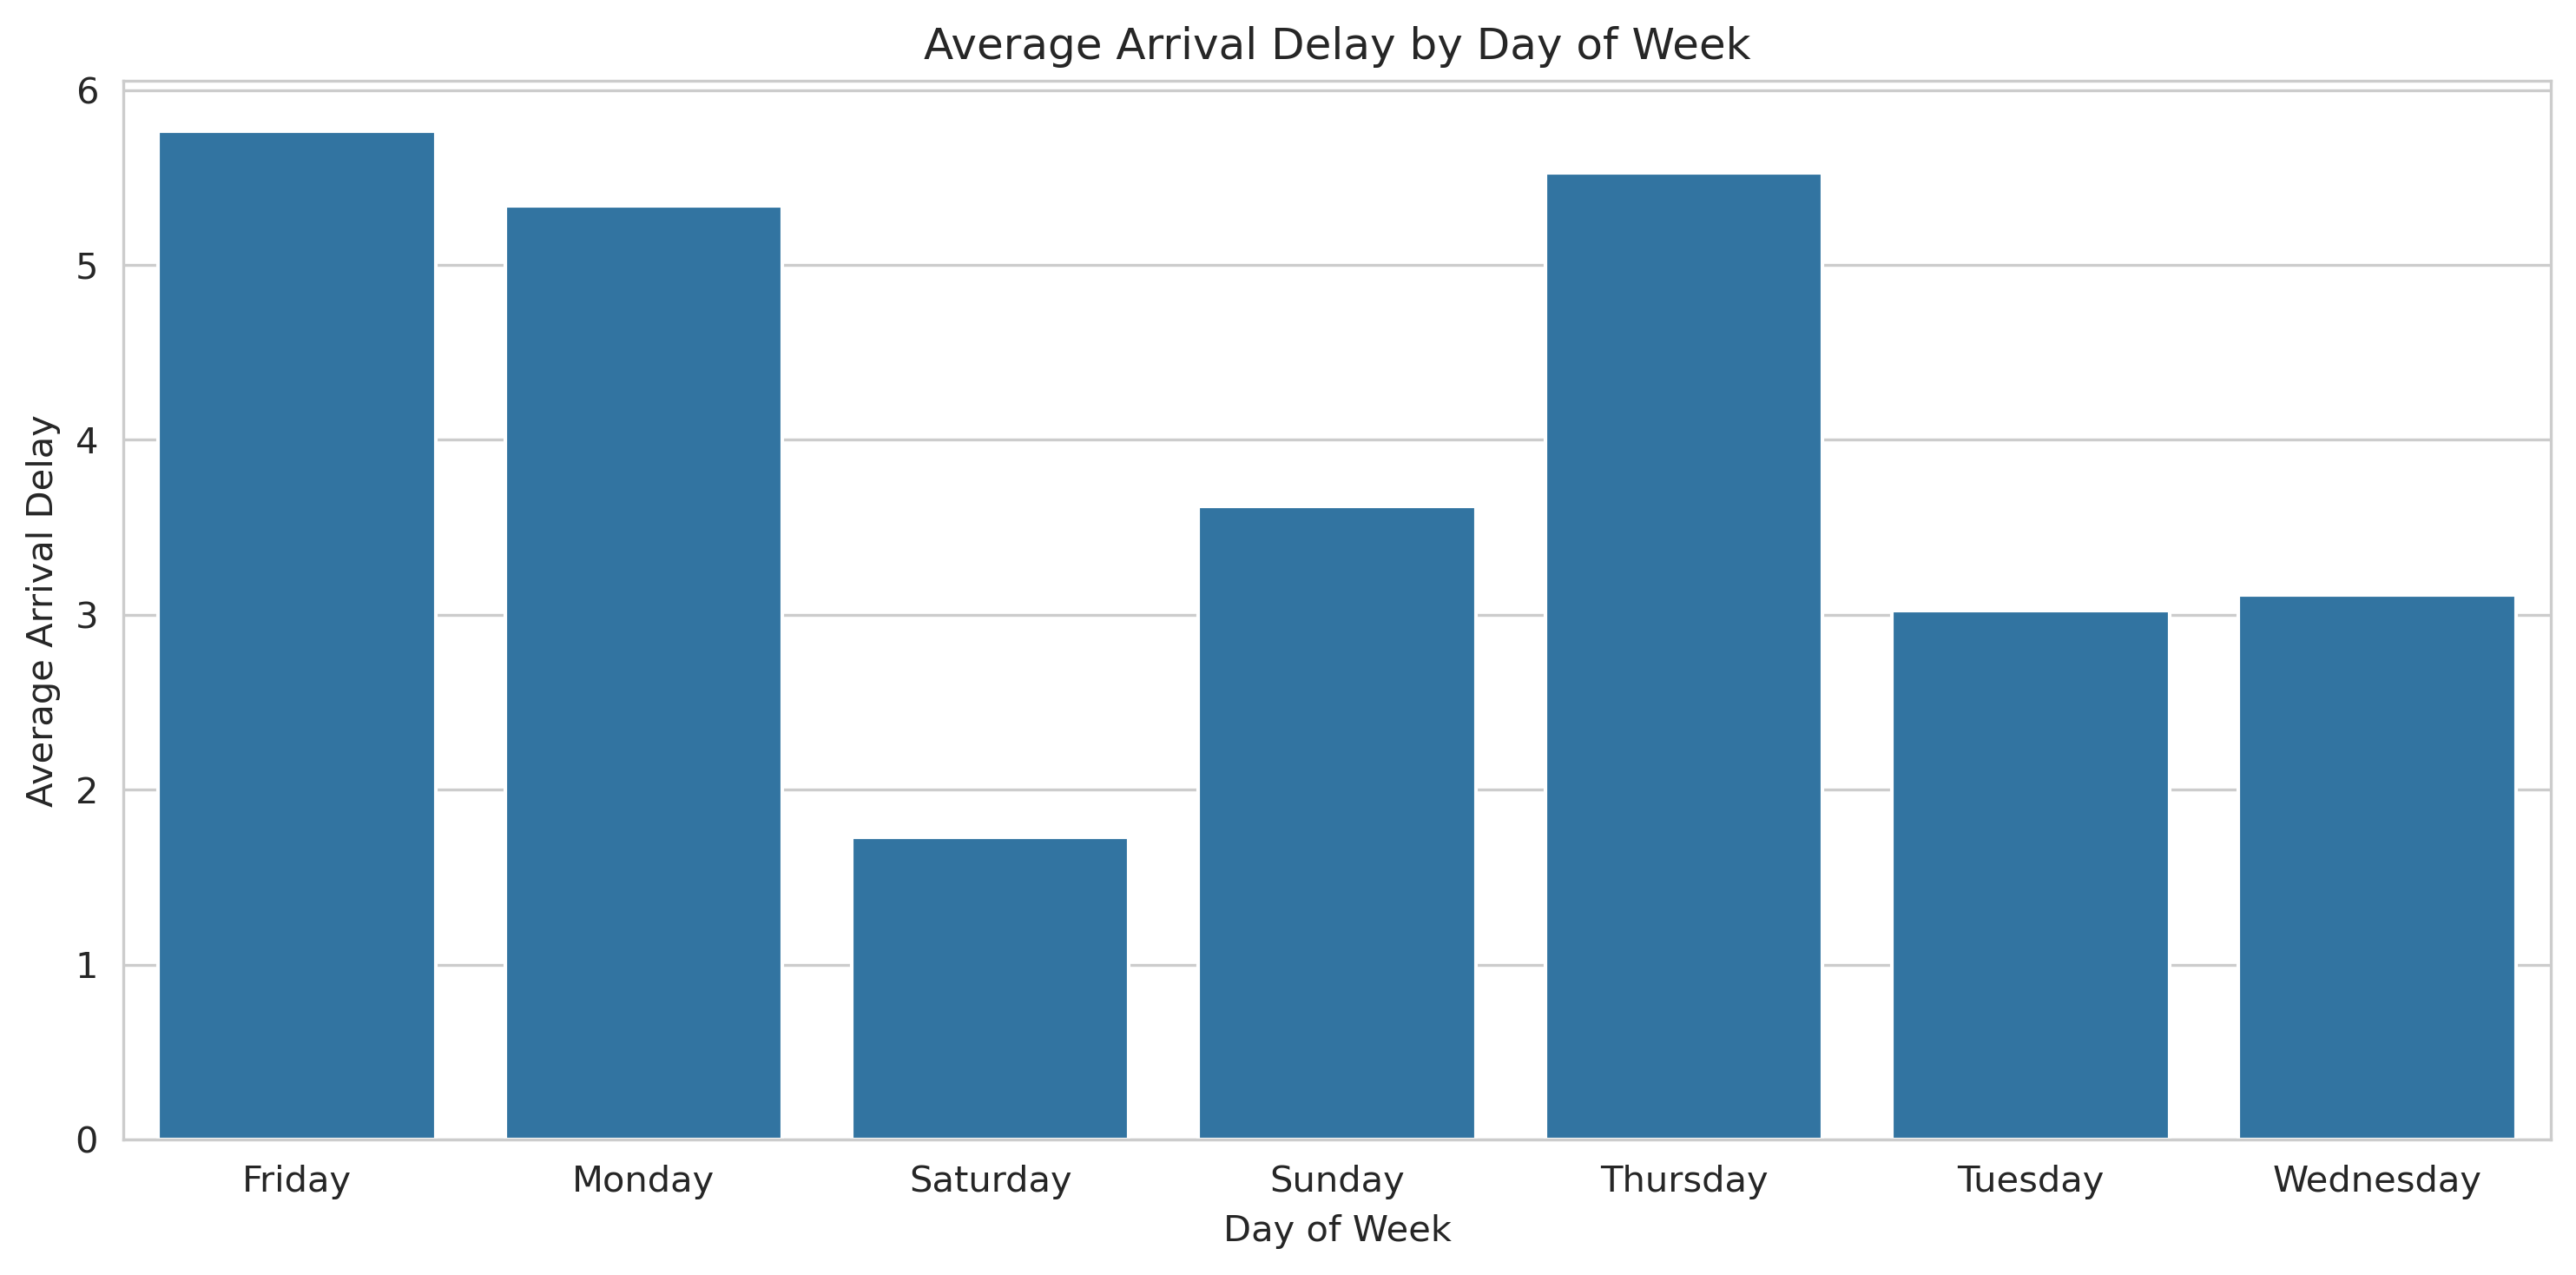
\includegraphics[width=0.85\textwidth]{figures/dow_delay.png}
    \caption{Average arrival delay by day of week. Friday and Monday exhibit the highest average delays.}
\end{figure}

\begin{figure}[H]
    \centering
    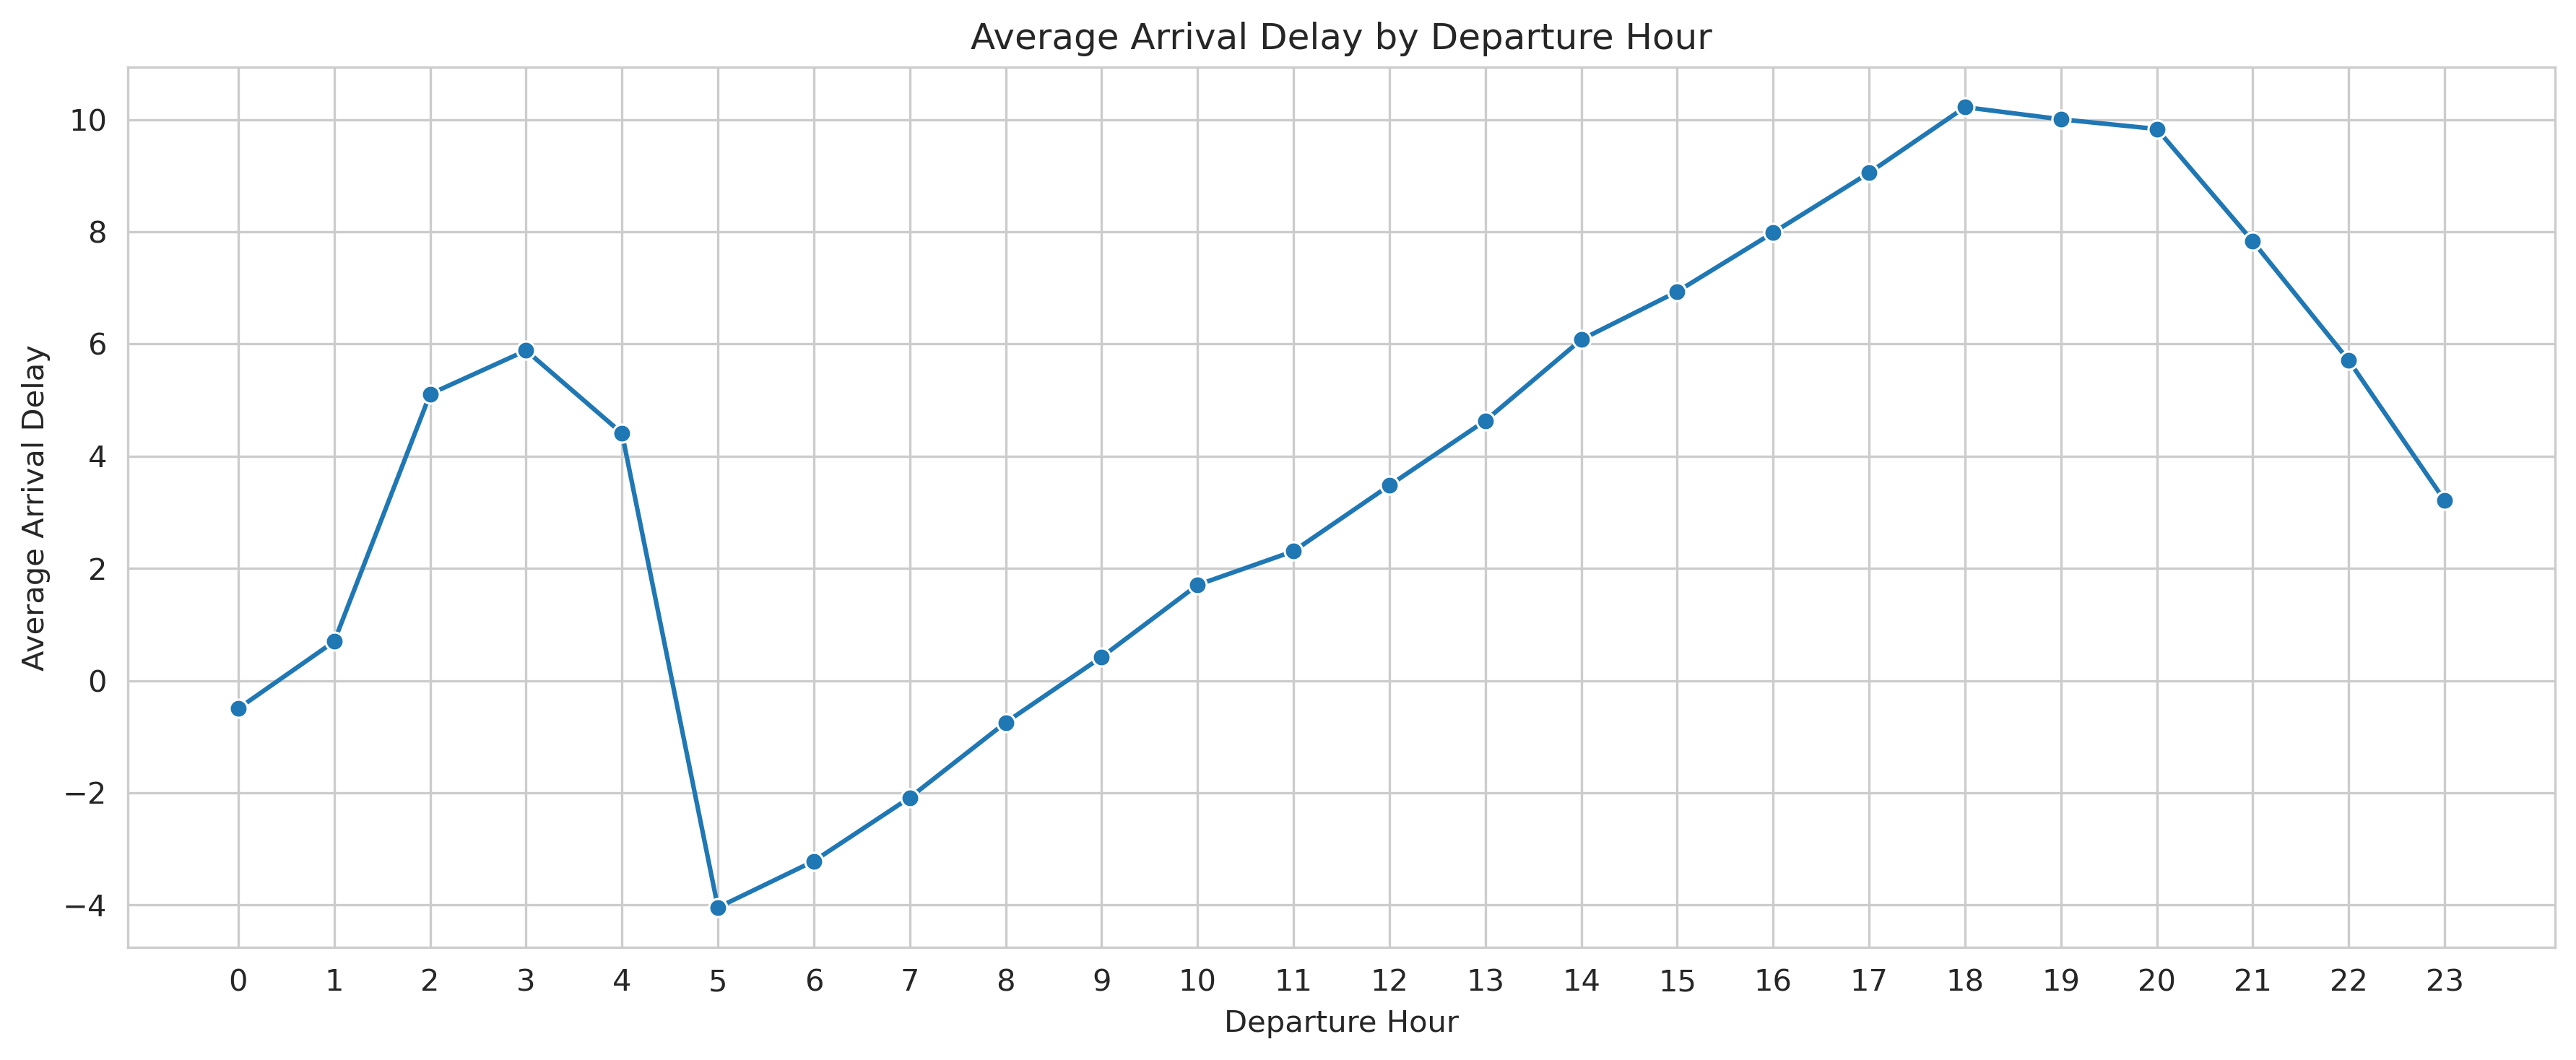
\includegraphics[width=0.85\textwidth]{figures/hourly_delay.png}
    \caption{Average arrival delay by scheduled departure hour. Delays increase throughout the day, peaking in the evening hours.}
\end{figure}

Key temporal findings:
\begin{itemize}
    \item \textbf{Day of week:} Friday and Monday have the highest average delays, likely due to increased business travel demand
    \item \textbf{Hour of day:} Delays increase progressively from morning to evening, suggesting delay propagation throughout the day
    \item \textbf{Seasonality:} Summer months (June--August) have higher flight volumes and delays
\end{itemize}

\section{Carrier and Airport Performance}

\subsection{Carrier Delay Analysis}

\begin{figure}[H]
    \centering
    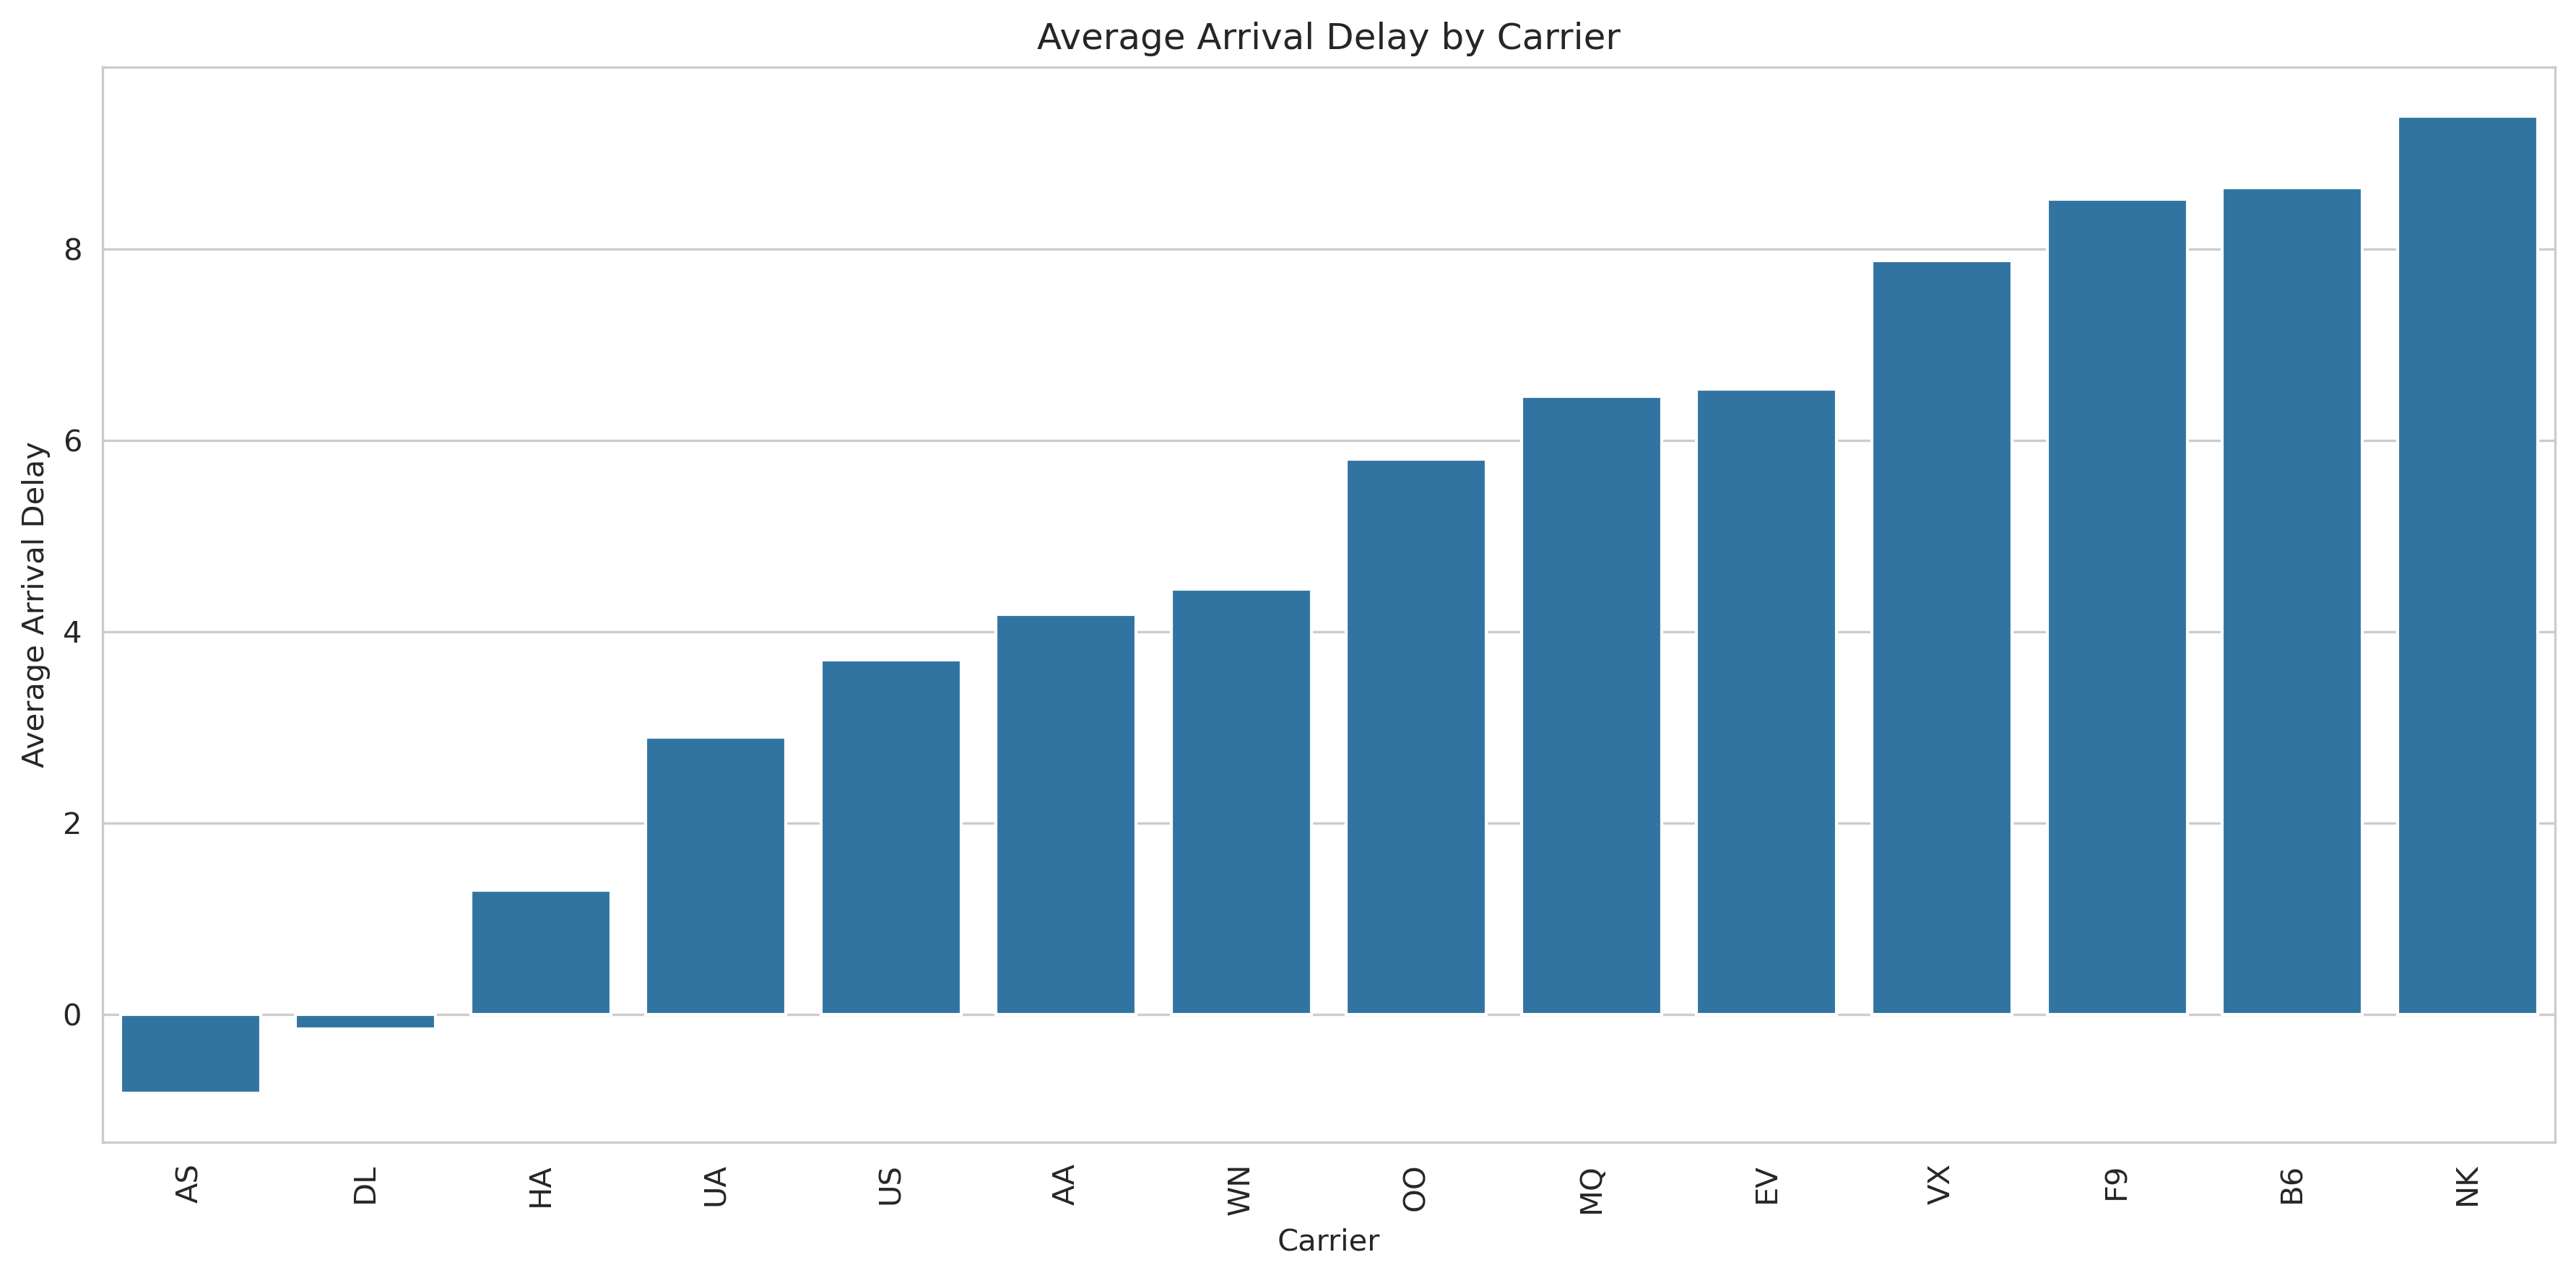
\includegraphics[width=0.85\textwidth]{figures/carrier_delay.png}
    \caption{Average arrival delay by carrier. Significant variation exists across airlines.}
\end{figure}

\begin{figure}[H]
    \centering
    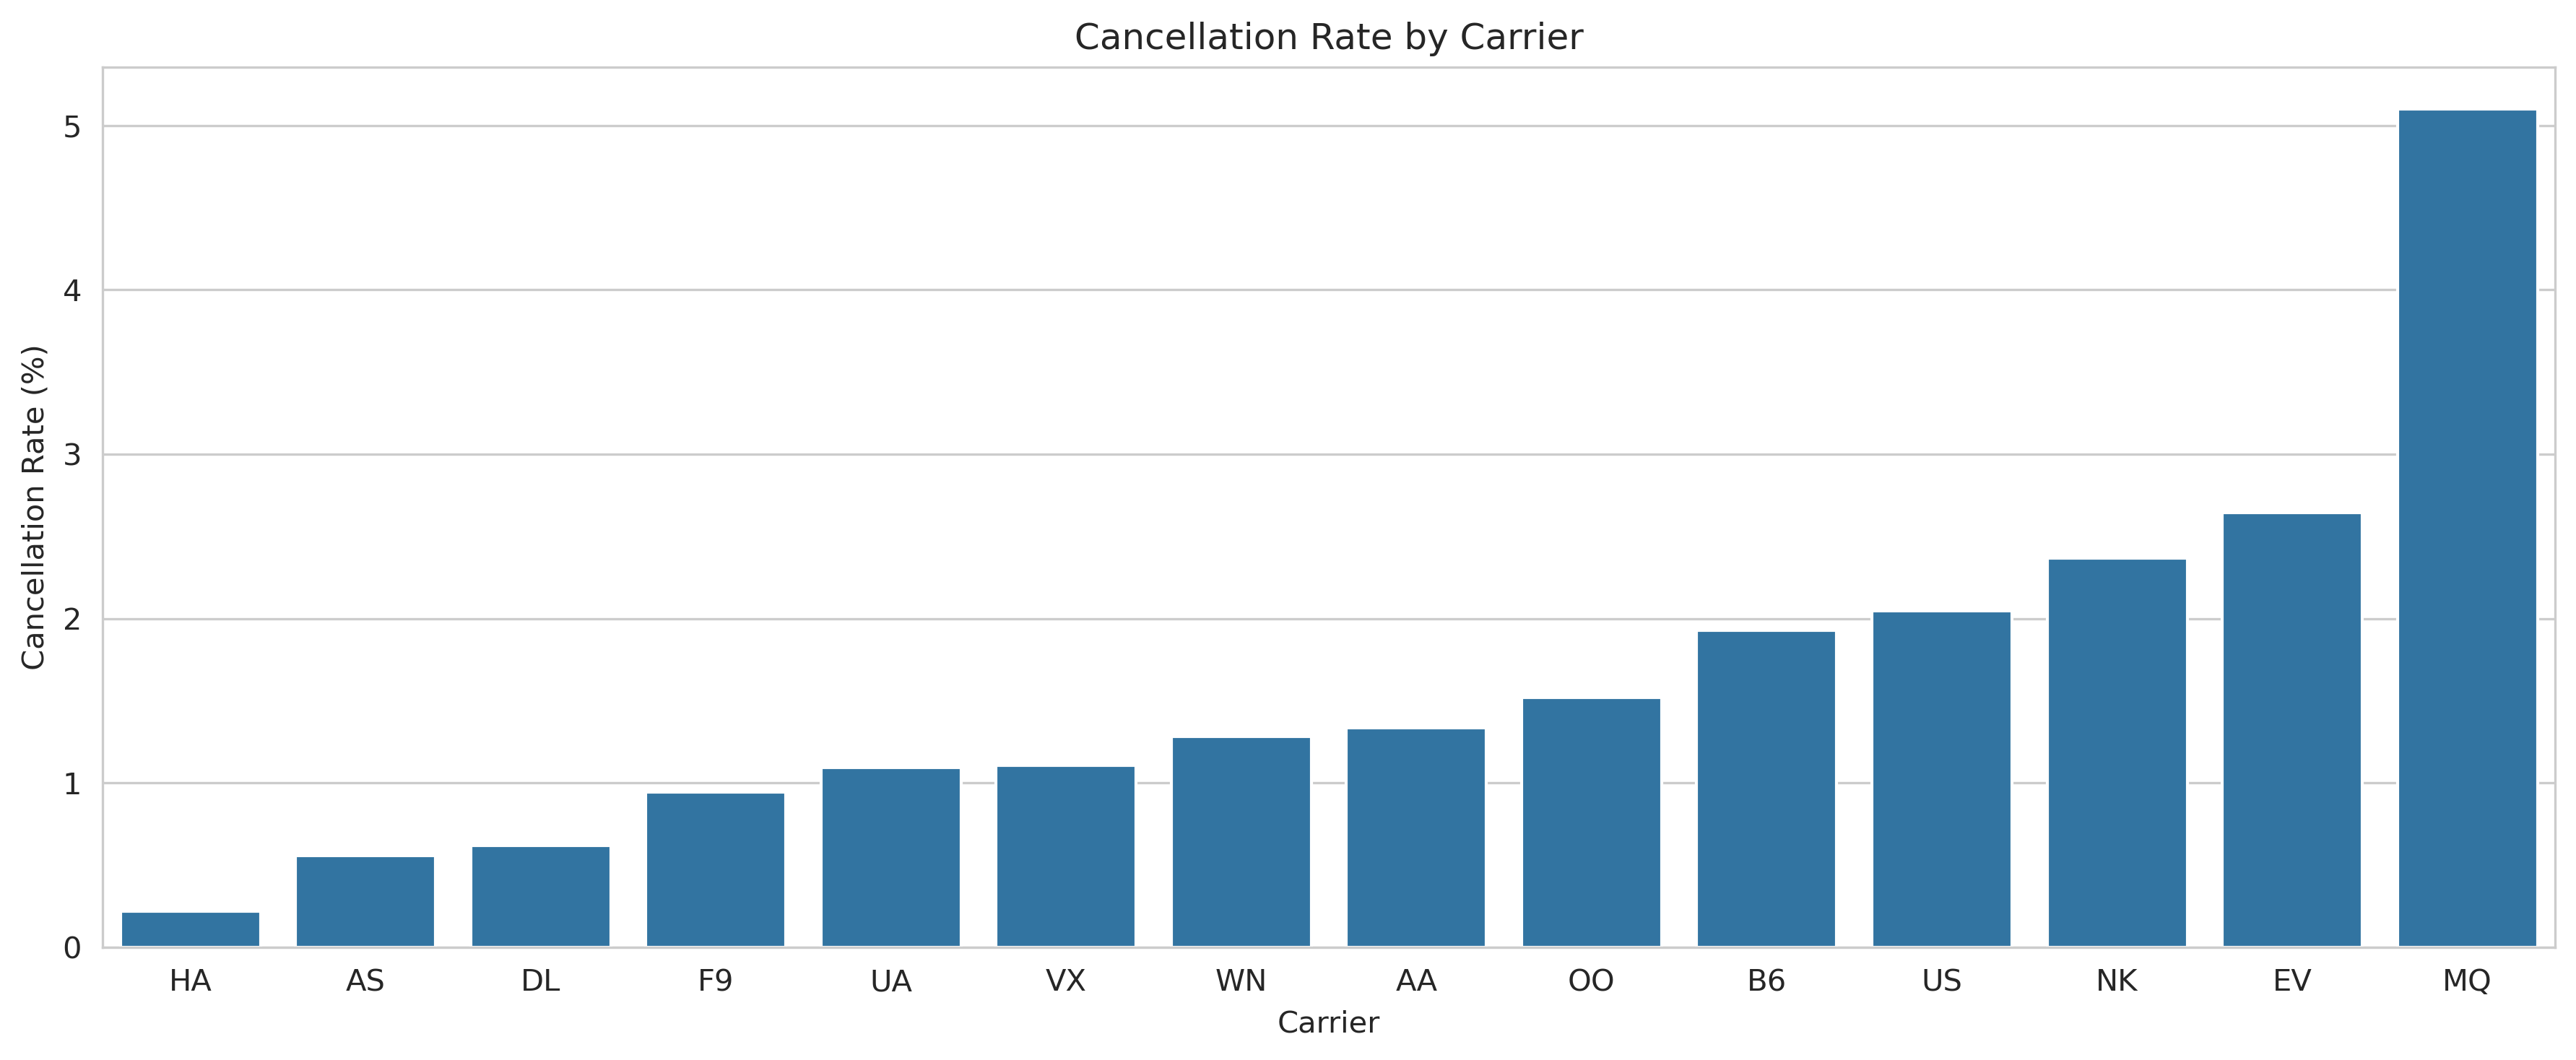
\includegraphics[width=0.85\textwidth]{figures/carrier_cancel_rate.png}
    \caption{Cancellation rate by carrier. Some regional carriers exhibit disproportionately high cancellation rates.}
\end{figure}

\subsection{Airport Delay Analysis}

\begin{figure}[H]
    \centering
    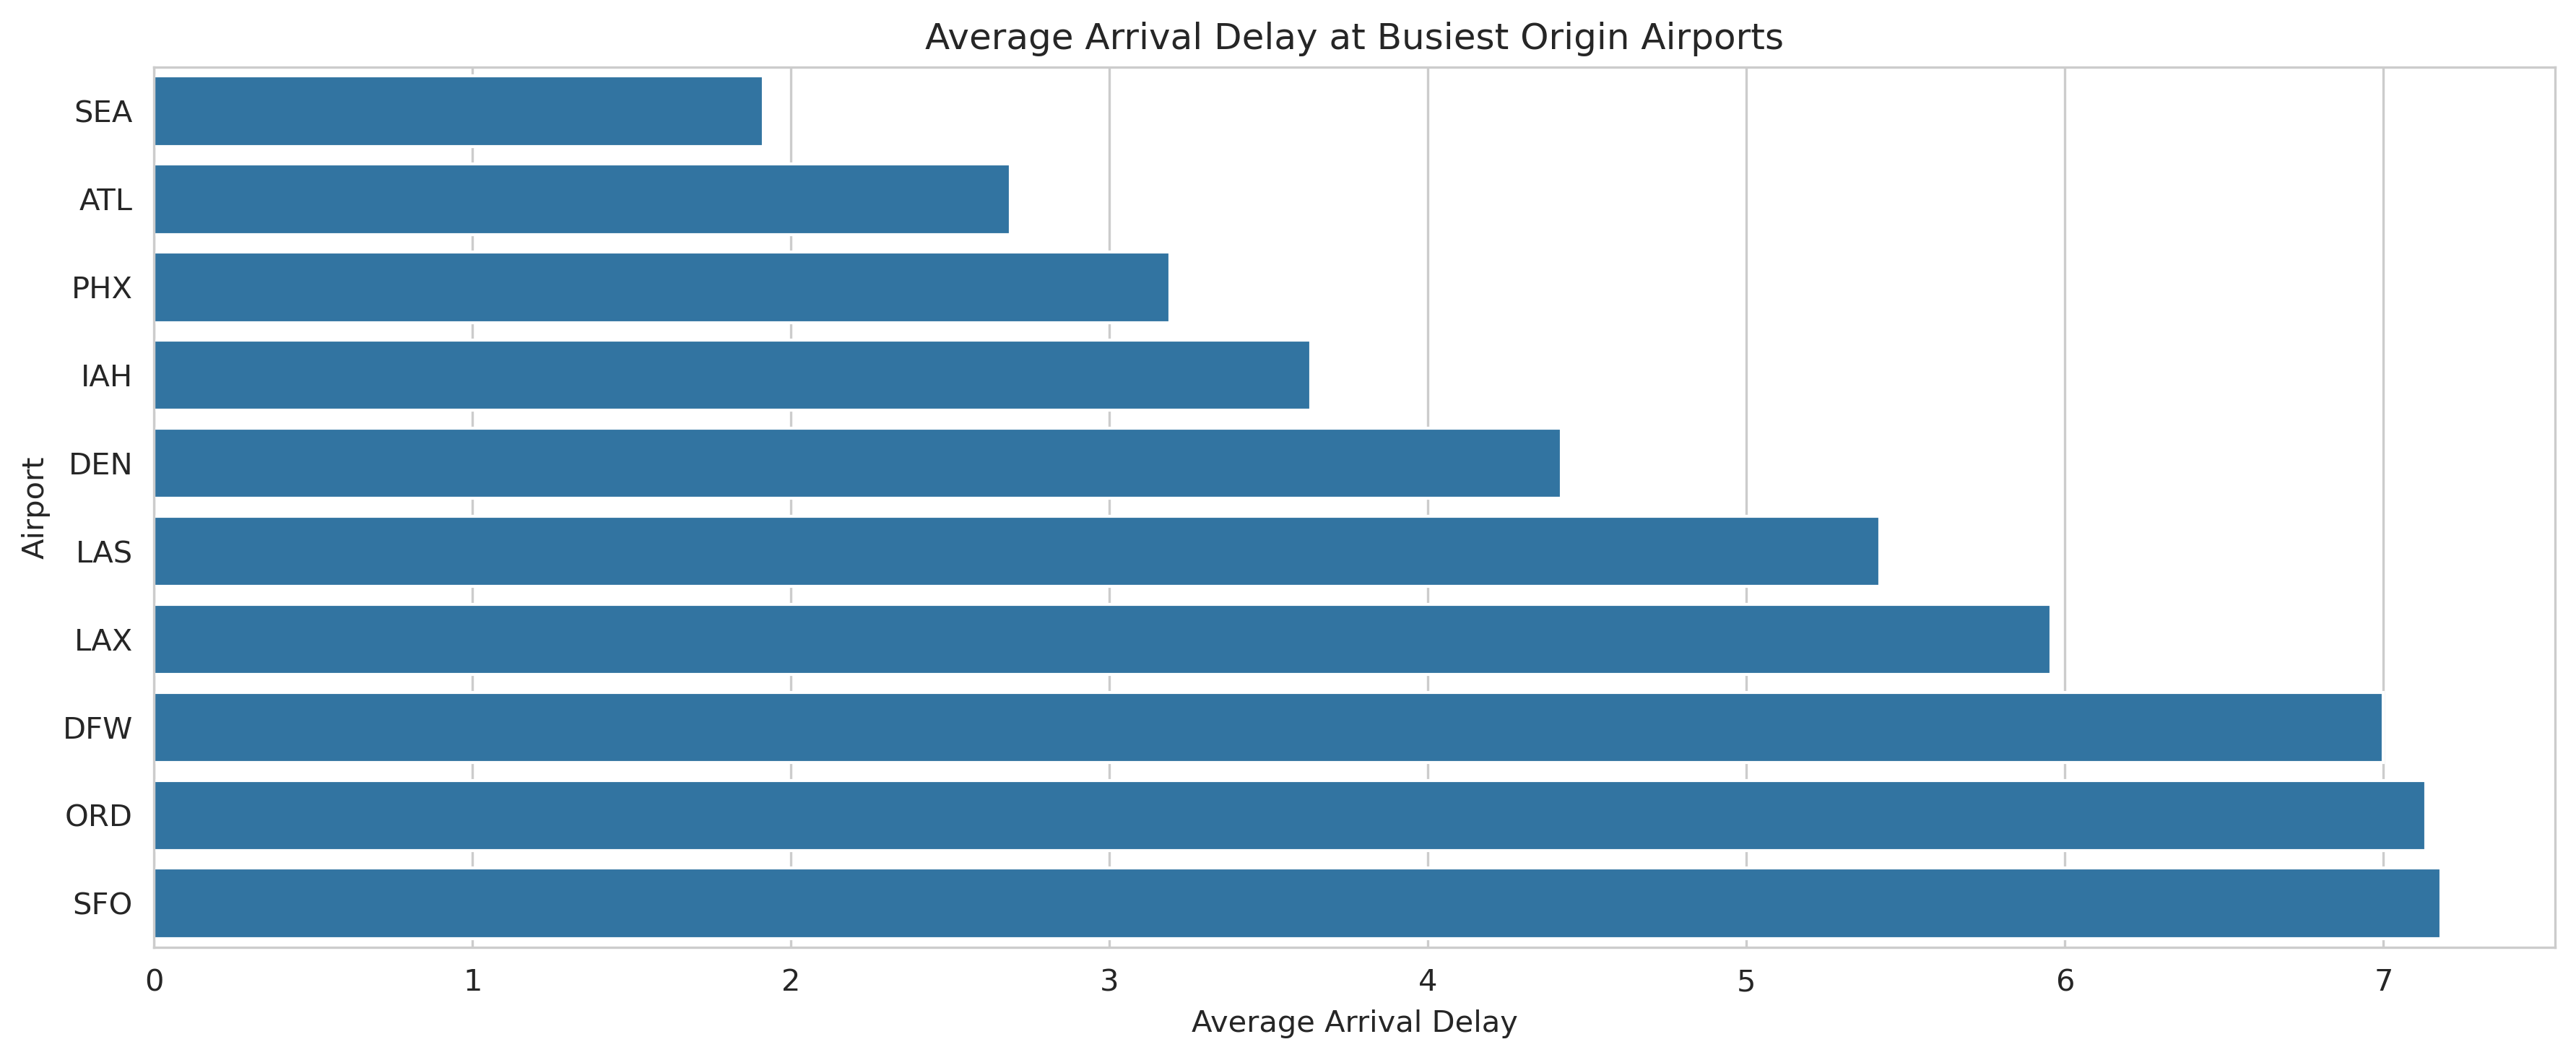
\includegraphics[width=0.85\textwidth]{figures/airport_delays.png}
    \caption{Average arrival delay at the busiest origin airports. Traffic volume alone does not determine delay severity.}
\end{figure}

\section{Bivariate Analysis}

\subsection{Departure Delay vs Arrival Delay}

\begin{figure}[H]
    \centering
    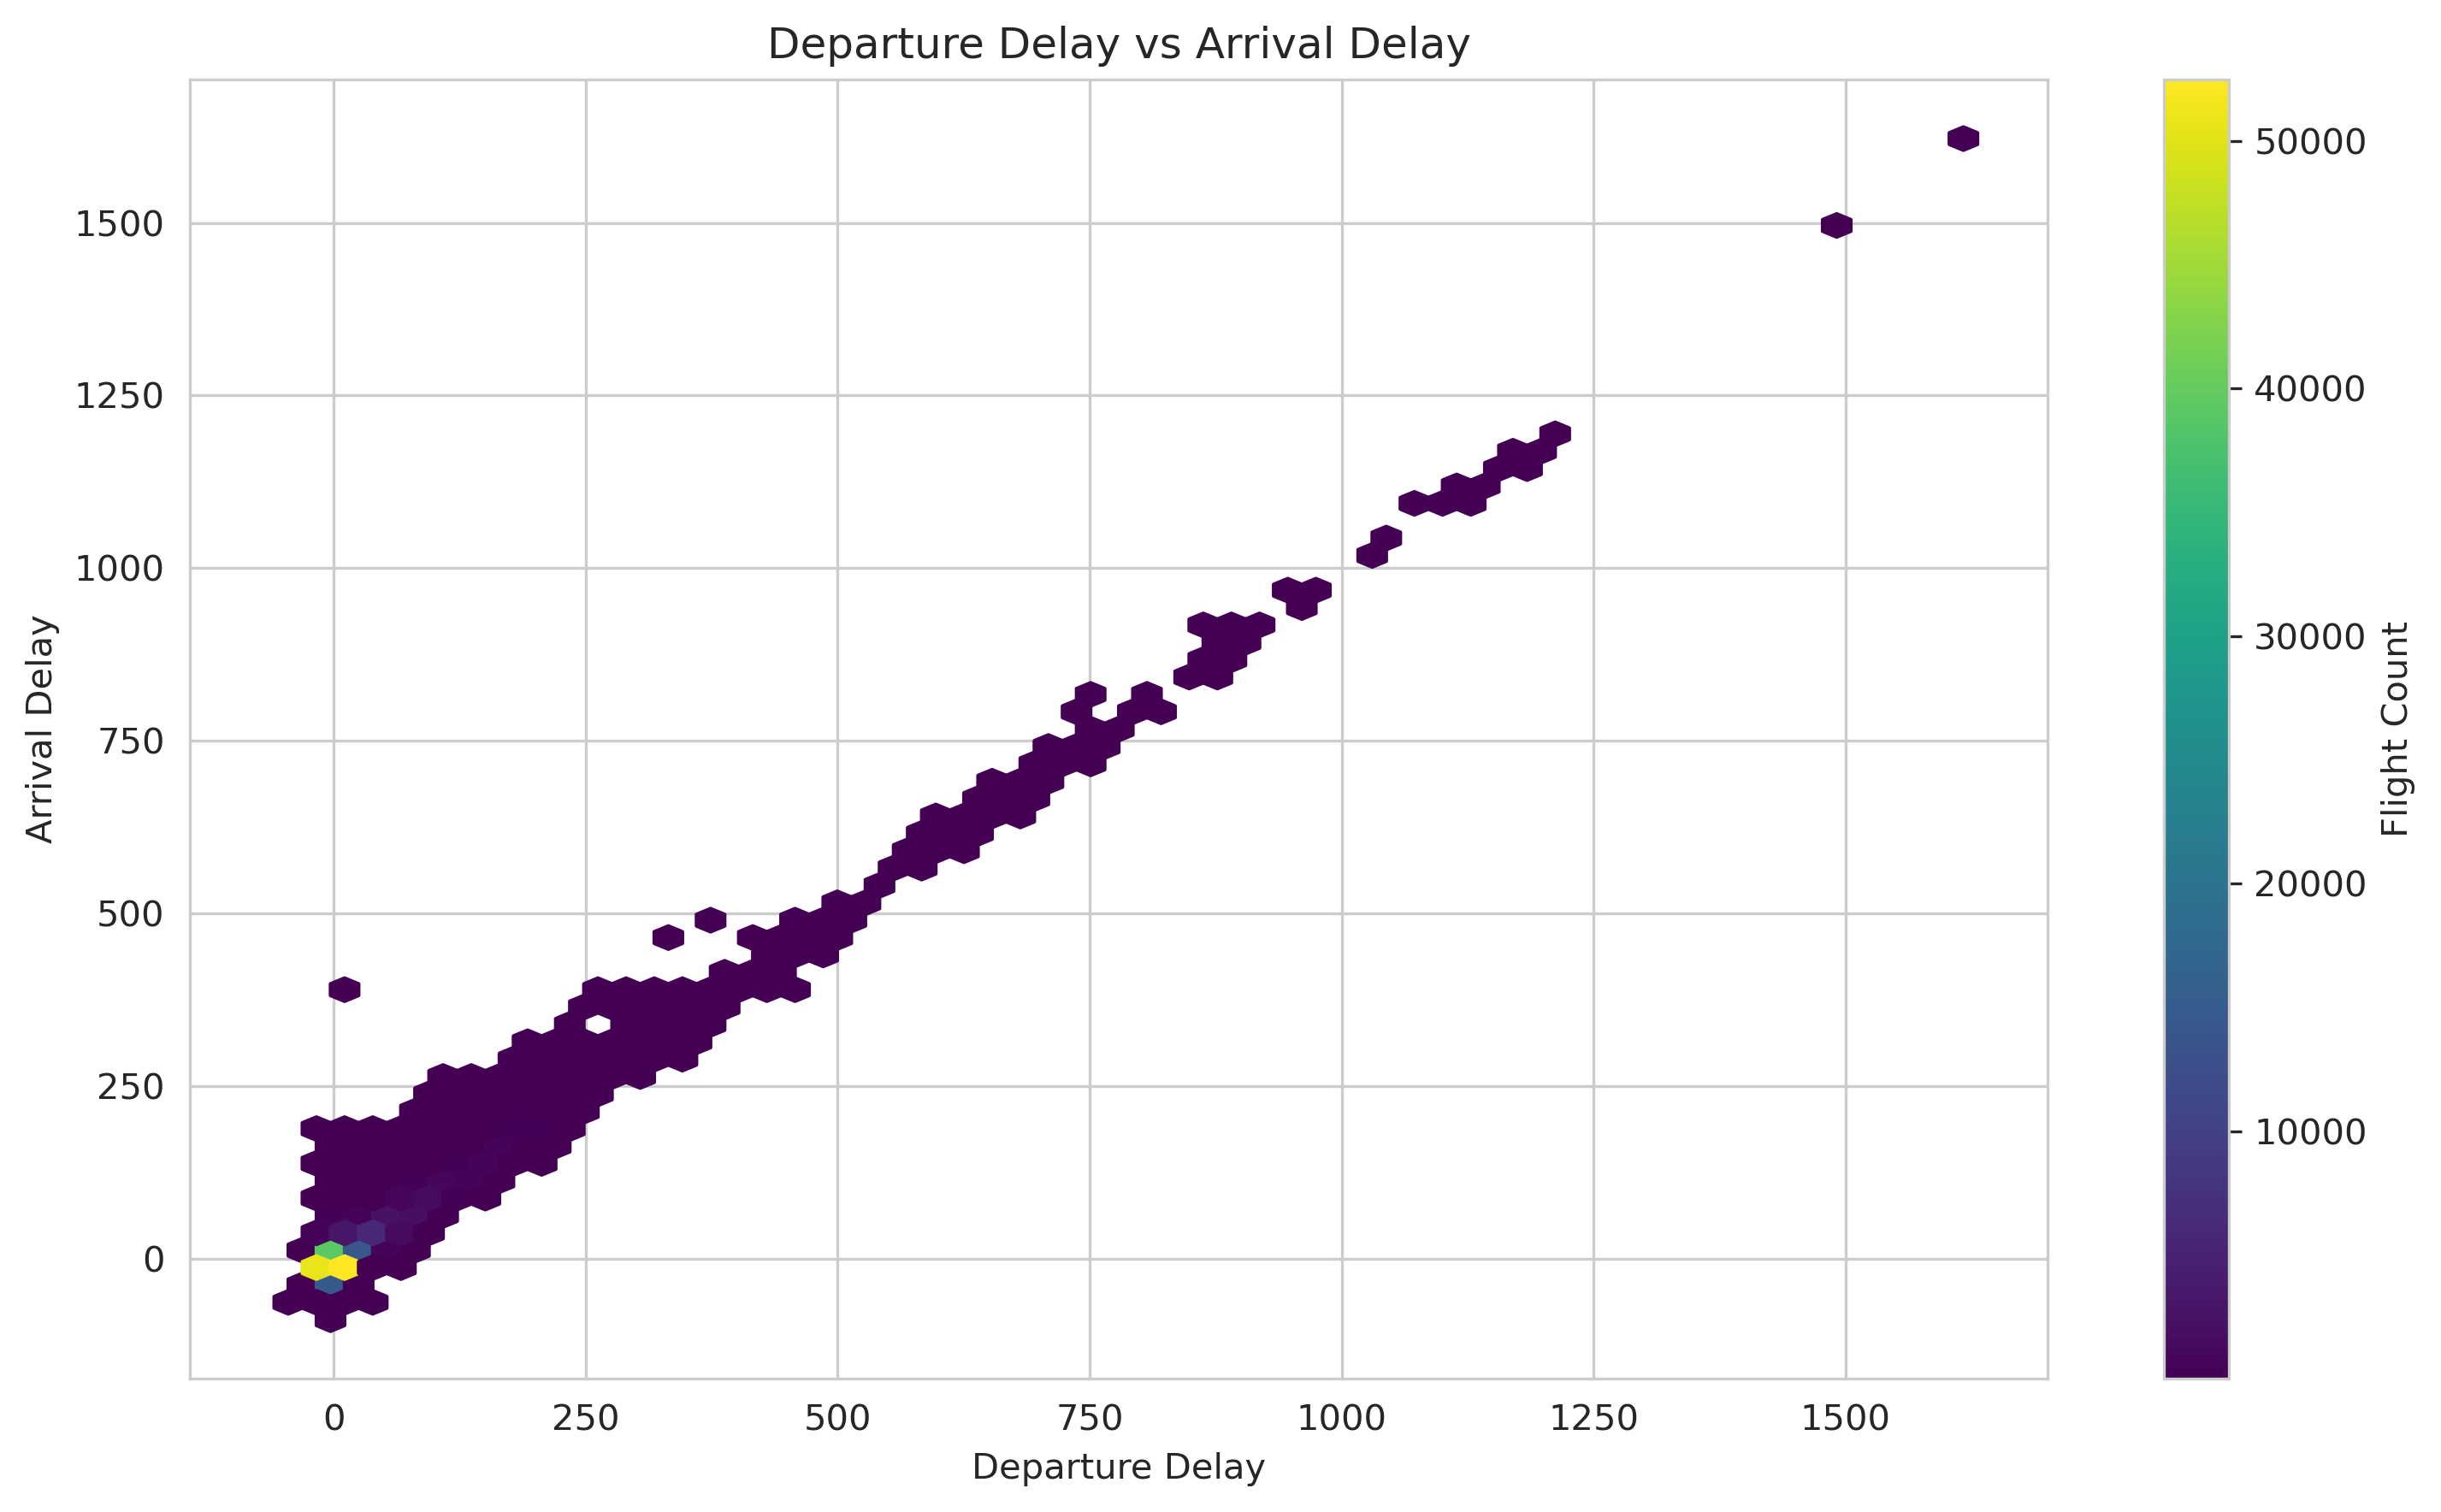
\includegraphics[width=0.85\textwidth]{figures/dep_arr_hexbin.png}
    \caption{Hexbin density plot of departure delay vs arrival delay. A strong linear relationship is evident ($\rho = 0.95$).}
\end{figure}

The correlation coefficient between departure delay and arrival delay is approximately 0.95, indicating that departure delays almost entirely propagate to arrival delays.

\subsection{Distance vs Arrival Delay}

\begin{figure}[H]
    \centering
    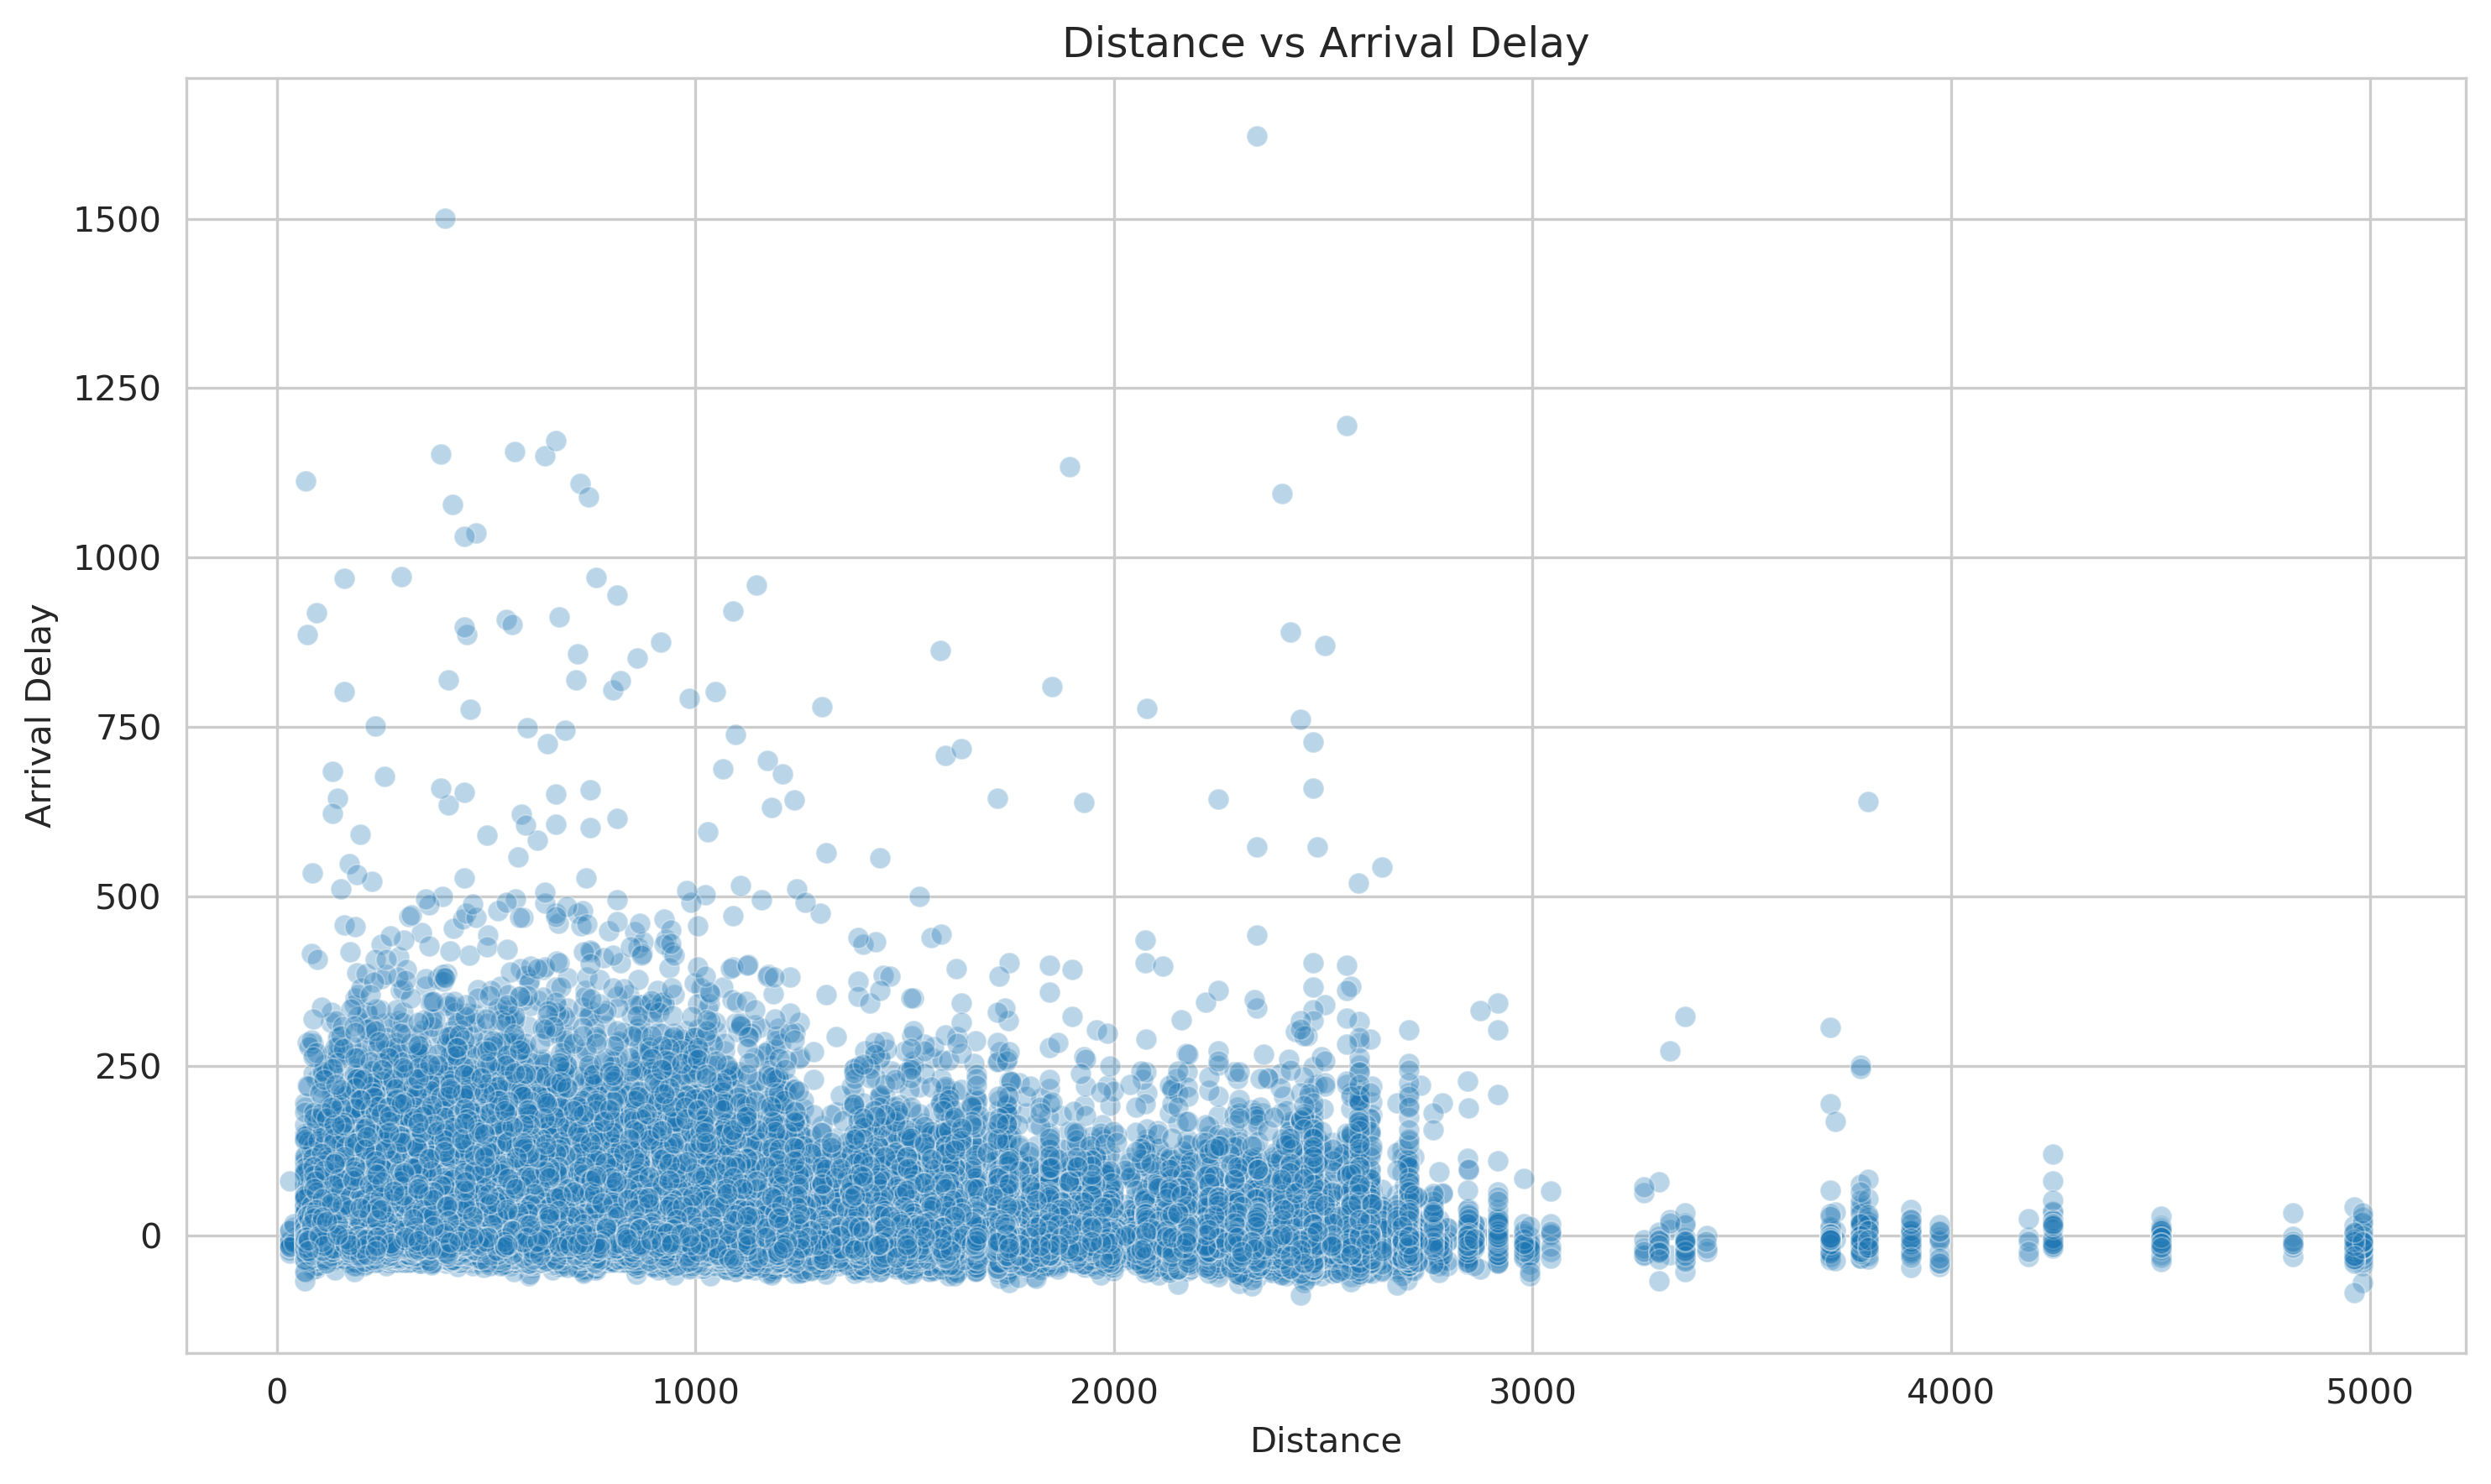
\includegraphics[width=0.85\textwidth]{figures/distance_delay.png}
    \caption{Scatter plot of flight distance vs arrival delay. No linear relationship is observed.}
\end{figure}

Flight distance shows negligible correlation with arrival delay, suggesting that longer flights are not inherently more prone to delays.

\section{Multivariate Analysis and Correlation}

\subsection{Correlation Matrix}

\begin{figure}[H]
    \centering
    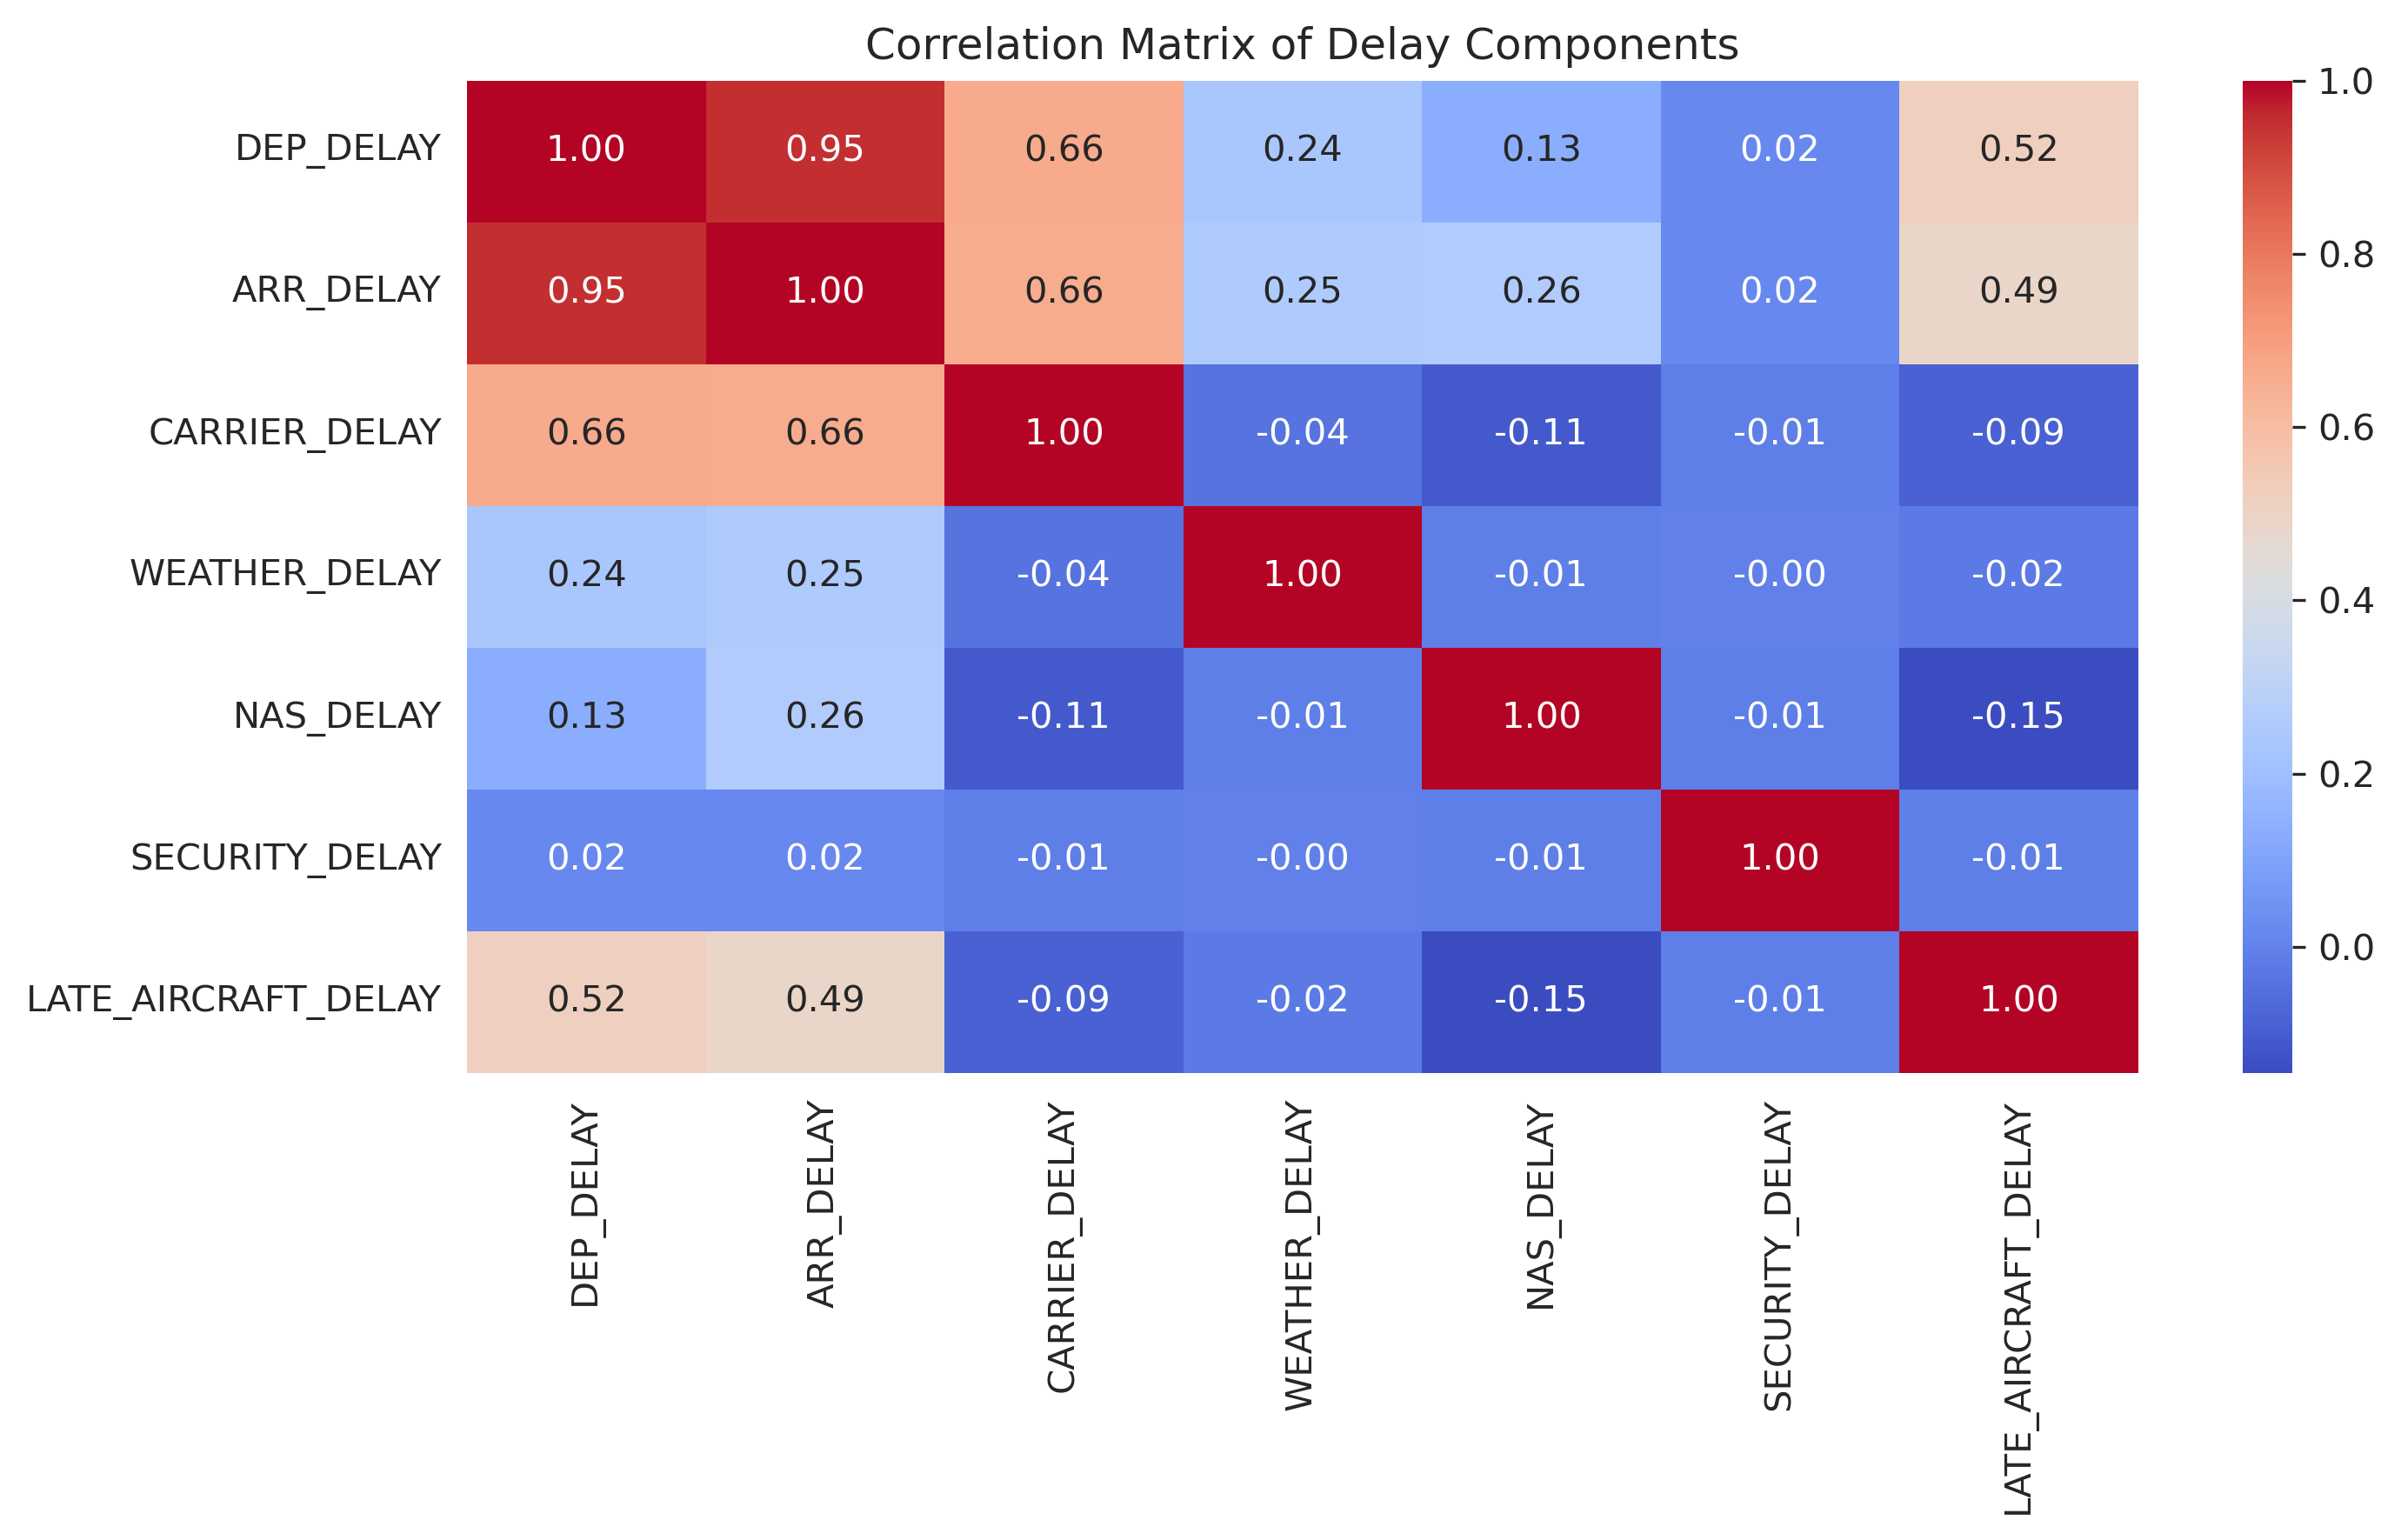
\includegraphics[width=0.85\textwidth]{figures/corr_heatmap.png}
    \caption{Correlation matrix of delay-related variables. Strong correlations exist between DEP\_DELAY, ARR\_DELAY, and LATE\_AIRCRAFT\_DELAY.}
\end{figure}

\subsection{Delay Cause Breakdown}

\begin{figure}[H]
    \centering
    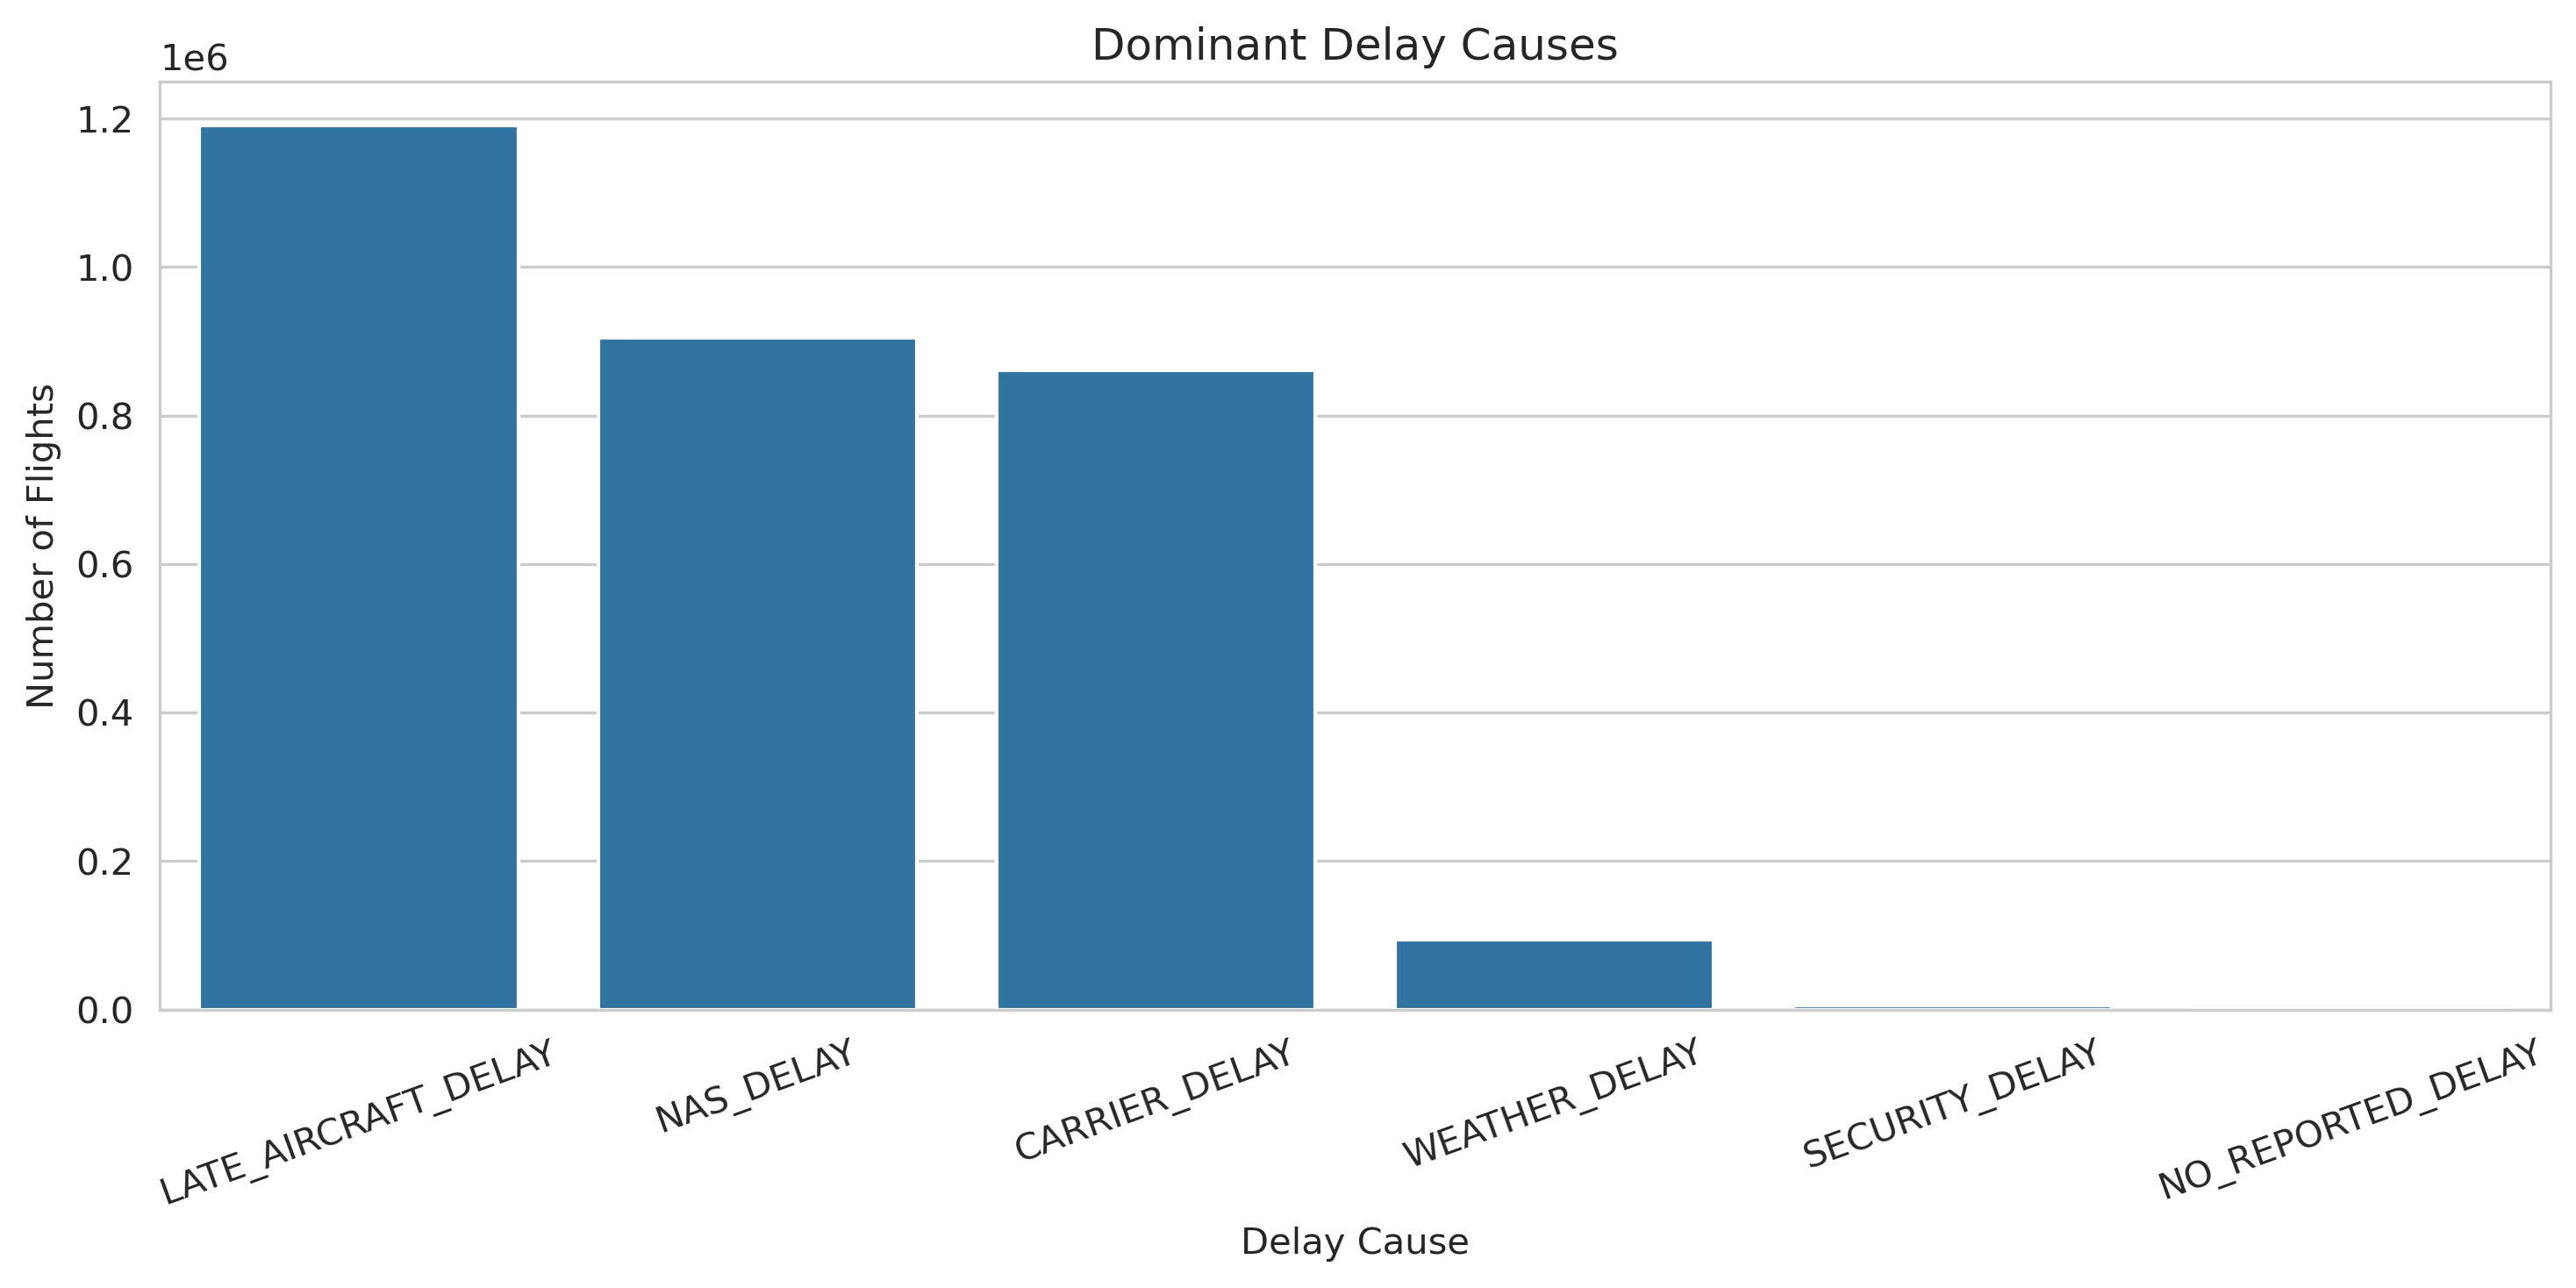
\includegraphics[width=0.85\textwidth]{figures/main_delay_cause.png}
    \caption{Dominant delay cause for delayed flights. Late aircraft delay is the most frequently reported primary cause.}
\end{figure}

The dominant delay category is \texttt{LATE\_AIRCRAFT\_DELAY}, confirming that delay propagation through the airline network is the primary mechanism behind flight disruptions. NAS delay and carrier delay are secondary contributors.

\subsection{Delay-Cancellation Relationship}

\begin{figure}[H]
    \centering
    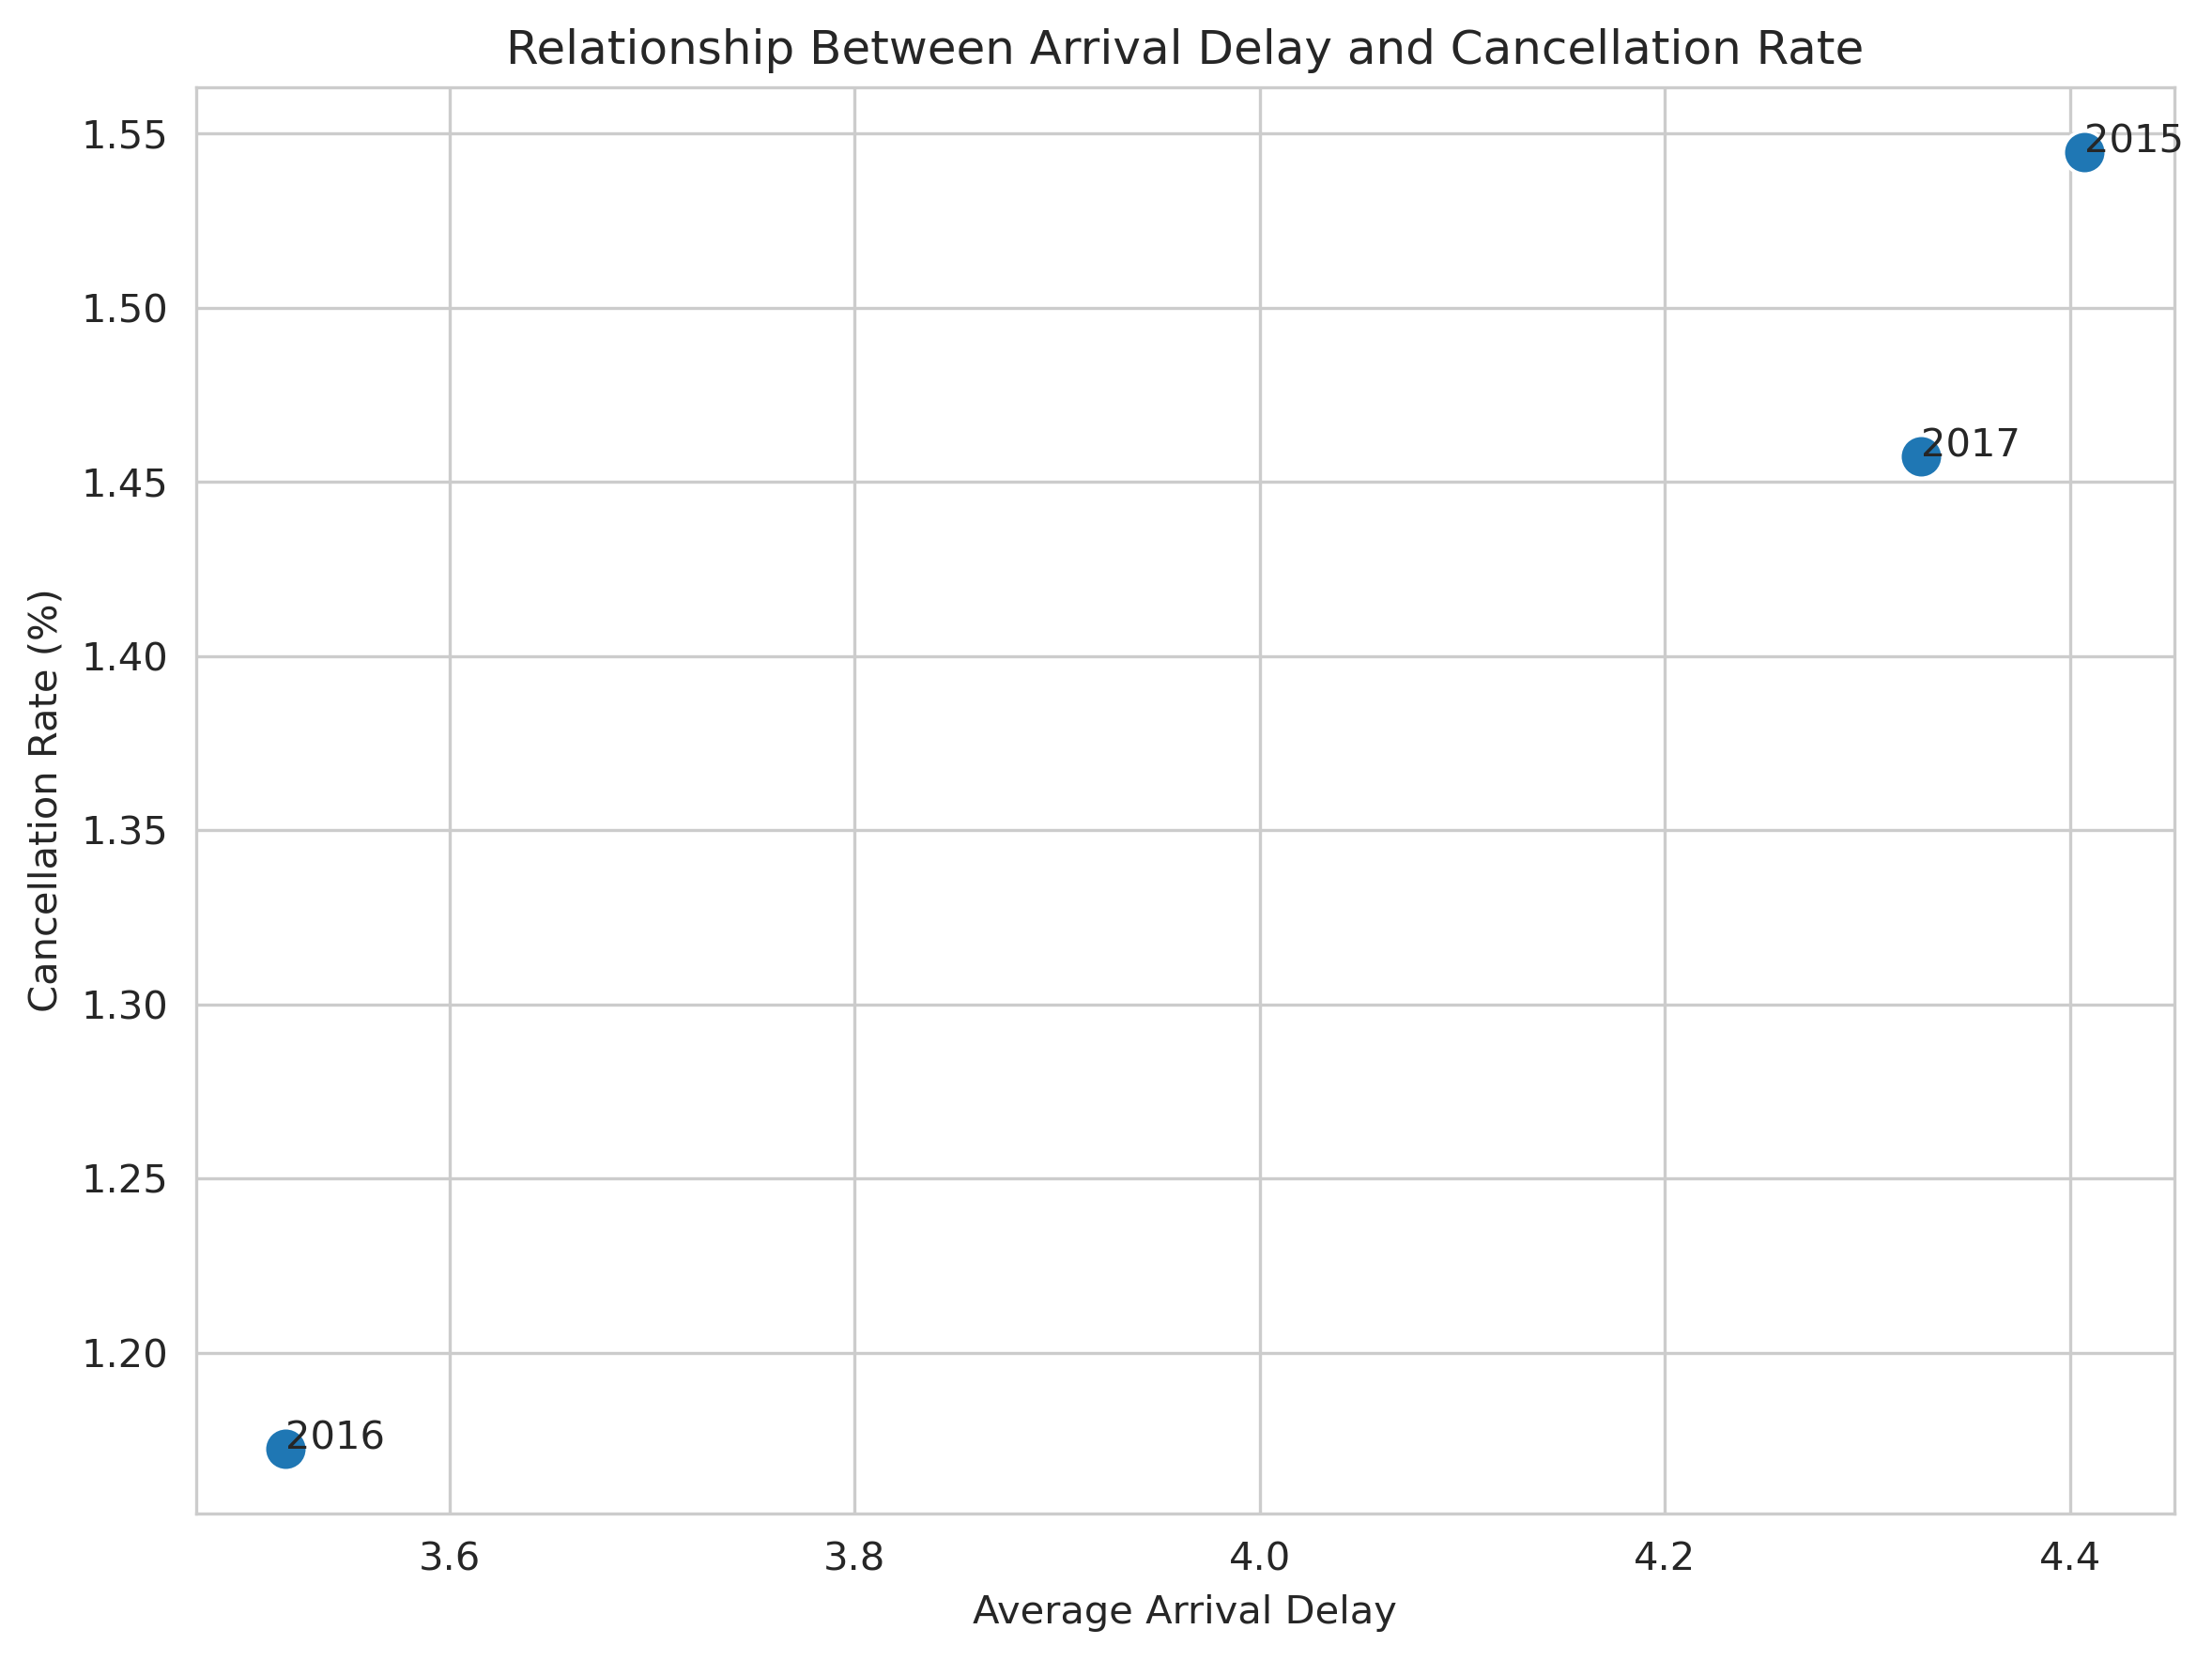
\includegraphics[width=0.85\textwidth]{figures/delay_cancel_scatter.png}
    \caption{Relationship between average arrival delay and cancellation rate by year.}
\end{figure}

\section{Discussion}

\subsection{Key Findings}

\begin{enumerate}
    \item \textbf{Delay propagation dominates:} The strong correlation ($\rho = 0.95$) between departure and arrival delays, combined with late aircraft delay being the most common primary cause, indicates that the U.S. domestic flight system is highly interconnected. Delays cascade through the network as aircraft, crew, and schedules are tightly coupled.

    \item \textbf{Temporal patterns:} Delays accumulate throughout the day, peaking in evening hours. This suggests that early-morning delays, though small, compound over successive flight legs.

    \item \textbf{Carrier heterogeneity:} Significant variation exists across airlines in both average delay and cancellation rate. This reflects differences in operational strategies, network structures, and schedule buffers.

    \item \textbf{Airport effects:} Traffic volume alone does not predict delay severity, suggesting that airport-specific factors (infrastructure, weather patterns, air traffic control) play important roles.

    \item \textbf{Distance independence:} Flight distance has minimal impact on delay probability or severity, supporting the network propagation hypothesis.
\end{enumerate}

\subsection{Limitations}

\begin{itemize}
    \item This analysis is purely descriptive and does not model causal relationships
    \item External factors (weather data, air traffic control logs) were not included
    \item Delay cause data is missing for approximately 82\% of flights, limiting causal analysis
    \item Only three years of data were analyzed; longer-term trends may differ
    \item The dataset does not include passenger-level impact metrics
\end{itemize}

\section{Conclusion}

This exploratory data analysis of 17 million U.S. domestic flights (2015--2017) reveals that airline delays are primarily driven by operational propagation effects rather than external factors. The near-perfect correlation between departure and arrival delays, the dominance of late aircraft delay as a causal factor, and the accumulation of delays throughout the day all point toward a system where disruptions cascade through interconnected schedules.

These findings have practical implications for airlines and passengers. Schedule optimization, buffer management, and proactive delay mitigation on early-morning flights could reduce the ripple effects that lead to afternoon and evening disruptions. Future work could extend this analysis with predictive models, incorporate external weather data, and examine the impact of delays on passenger itineraries.

\appendix
\section{Appendix}

\subsection{Code Repository}

The complete analysis code, including data loading, preprocessing, visualization generation, and statistical summaries, is available in the Jupyter notebook \texttt{eda.ipynb}. All figures were generated using \texttt{generate\_figures.py} and are stored in the \texttt{figures/} directory.

The full project is hosted on GitHub: \url{https://github.com/fermow/SBU-Data-Science-2026}

\subsection{Variable Description}

\begin{table}[H]
\centering
\begin{tabularx}{\textwidth}{l X}
\toprule
\textbf{Variable} & \textbf{Description} \\
\midrule
FL\_DATE & Flight date \\
OP\_CARRIER & Operating carrier IATA code \\
OP\_CARRIER\_FL\_NUM & Flight number \\
ORIGIN & Origin airport IATA code \\
DEST & Destination airport IATA code \\
CRS\_DEP\_TIME & Scheduled departure time \\
DEP\_TIME & Actual departure time \\
DEP\_DELAY & Departure delay (minutes) \\
TAXI\_OUT & Taxi-out time (minutes) \\
WHEELS\_OFF & Wheels-off time \\
WHEELS\_ON & Wheels-on time \\
TAXI\_IN & Taxi-in time (minutes) \\
CRS\_ARR\_TIME & Scheduled arrival time \\
ARR\_TIME & Actual arrival time \\
ARR\_DELAY & Arrival delay (minutes) \\
CANCELLED & Cancellation indicator \\
CANCELLATION\_CODE & Reason for cancellation \\
DIVERTED & Diversion indicator \\
CRS\_ELAPSED\_TIME & Scheduled elapsed time (minutes) \\
ACTUAL\_ELAPSED\_TIME & Actual elapsed time (minutes) \\
AIR\_TIME & Air time (minutes) \\
DISTANCE & Flight distance (miles) \\
CARRIER\_DELAY & Delay caused by carrier (minutes) \\
WEATHER\_DELAY & Delay caused by weather (minutes) \\
NAS\_DELAY & Delay caused by National Air System (minutes) \\
SECURITY\_DELAY & Delay caused by security (minutes) \\
LATE\_AIRCRAFT\_DELAY & Delay caused by late aircraft arrival (minutes) \\
\bottomrule
\end{tabularx}
\caption{Full variable descriptions}
\end{table}

\subsection{Technology Stack}

\begin{itemize}
    \item Python 3.13
    \item pandas 3.0
    \item matplotlib 3.10
    \item seaborn 0.13
    \item \LaTeX{} (pdf\LaTeX)
\end{itemize}

\end{document}
